\documentclass[12pt, a4paper]{report}

\usepackage[utf8]{inputenc}
\usepackage[T1]{fontenc}
\usepackage{amsmath}
\usepackage{amsfonts}
\usepackage{amssymb}
\usepackage{graphicx}
\usepackage{subcaption}
\usepackage{float}
\usepackage{hyperref}
\usepackage{xcolor}
\usepackage{tikz}
\usepackage{geometry}
\geometry{a4paper, margin=1in}

% Custom commands for highlighting
\newcommand{\highlight}[2]{\colorbox{#1!20}{$\displaystyle #2$}}
\newcommand{\impformula}[1]{\highlight{blue}{#1}}
\newcommand{\imppoint}[1]{\colorbox{green!10}{\textit{#1}}}

\title{Bachelor Thesis Report: Applications of Conformal Mapping}
\author{Manus AI}
\date{\today}

\begin{document}

\maketitle

\tableofcontents
\newpage

% Chapter 1: Introduction
\chapter{Introduction}

Conformal mapping is a powerful mathematical tool used to transform complex functions while preserving angles locally. This technique finds extensive applications in various fields of engineering and physics, particularly in solving boundary value problems that are otherwise intractable in their original domains. The primary advantage of conformal mapping lies in its ability to simplify complex geometries into more manageable standard regions, such as the upper half-plane or the unit disk, where solutions to physical problems are well-known.

\begin{figure}[H]
    \centering
    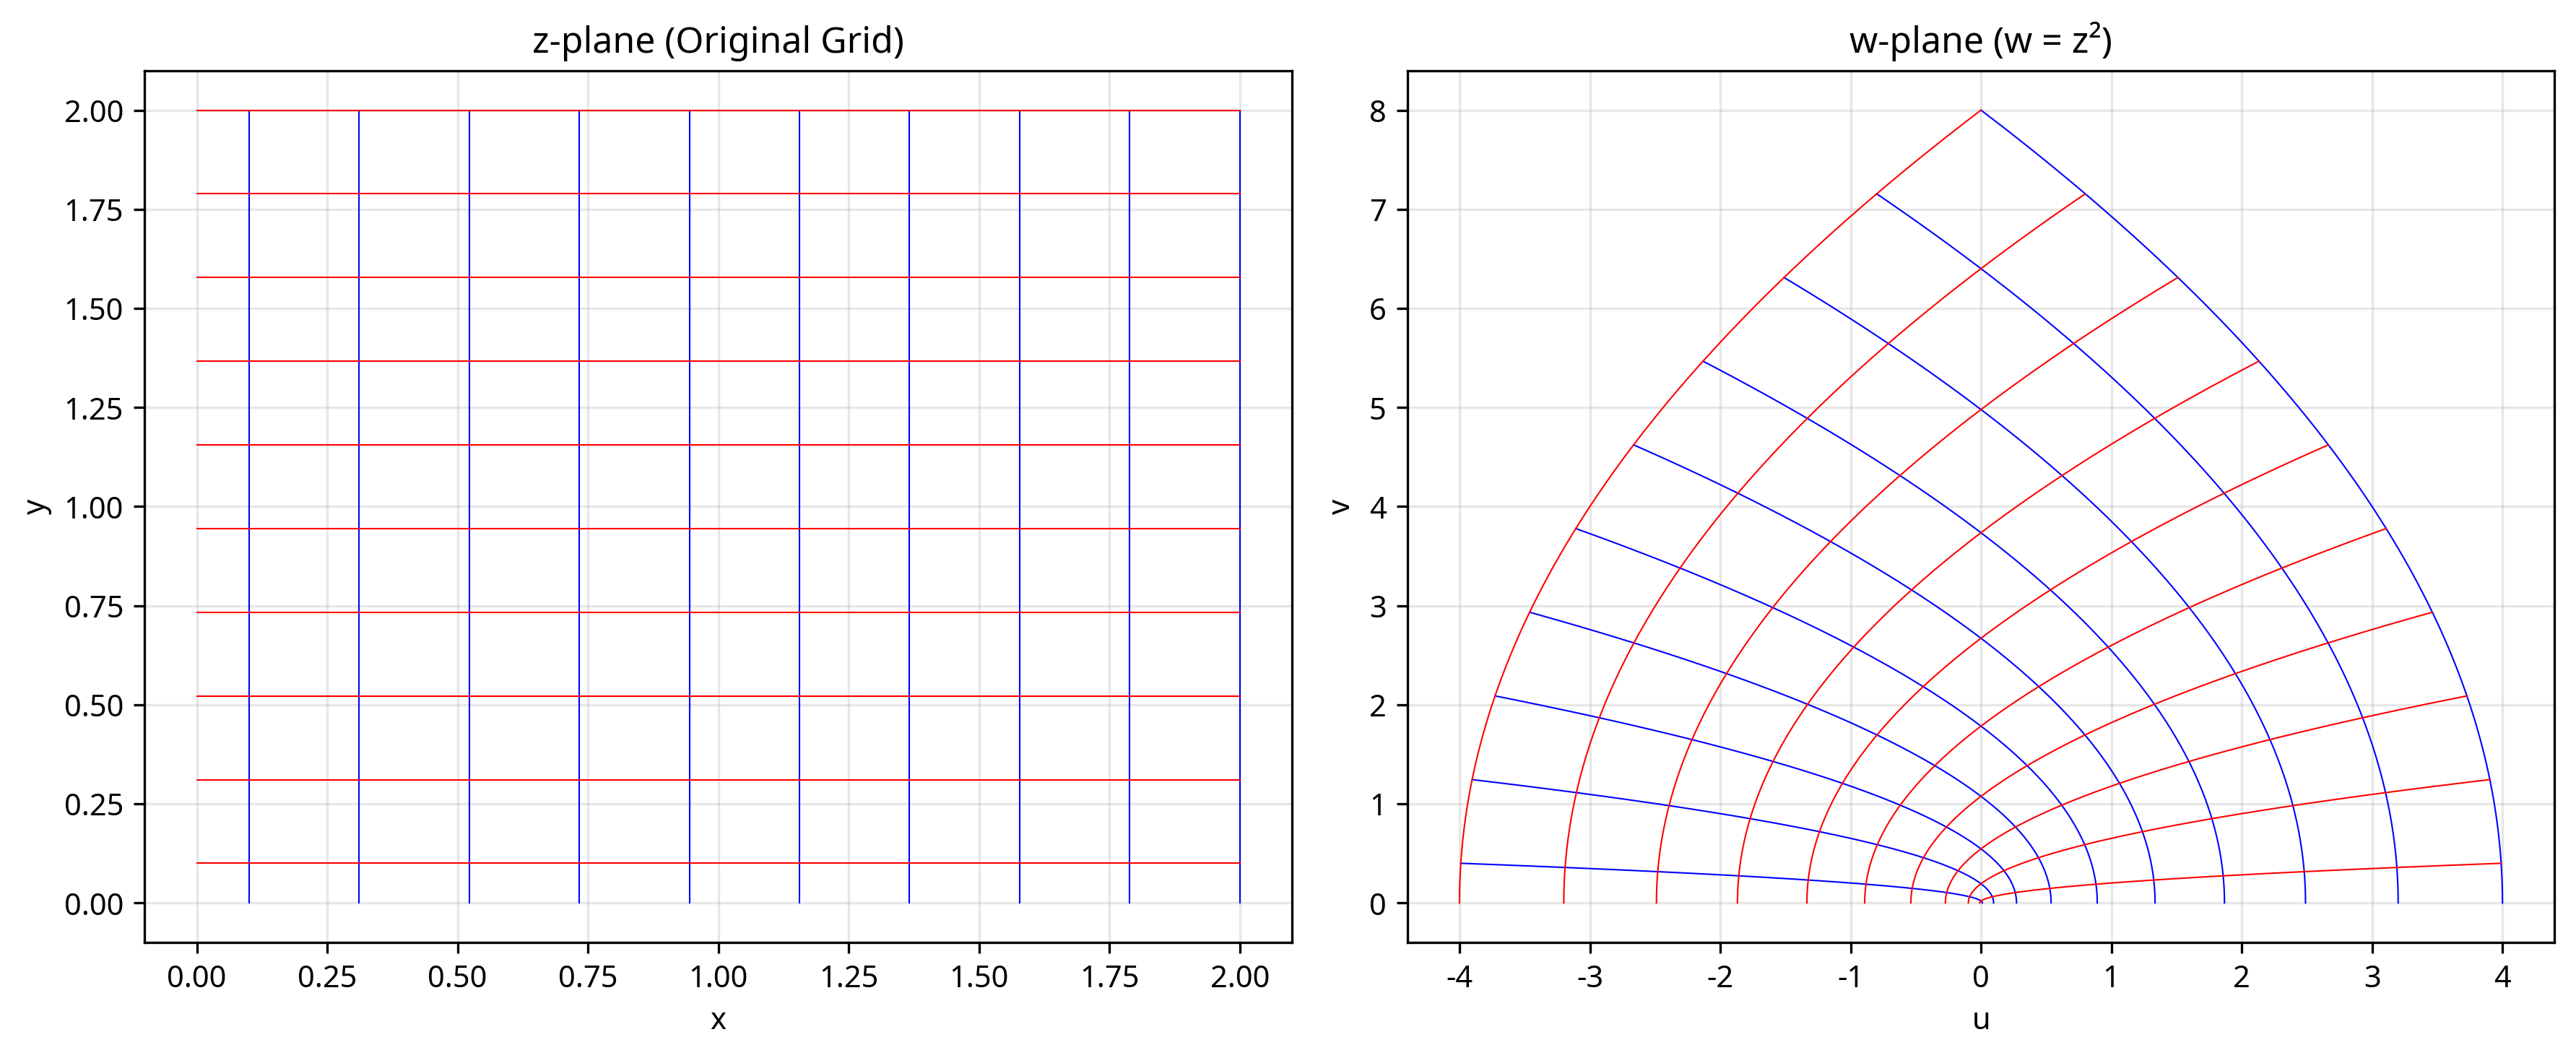
\includegraphics[width=0.8\textwidth]{diagrams/grid_transform_z2.png}
    \caption{Visualizing a conformal map $w = z^2$. Note how the grid lines remain orthogonal at every intersection, a defining property of conformal mappings.}
    \label{fig:grid_z2}
\end{figure}

This report delves into the applications of conformal mapping, with a particular focus on the Schwarz-Christoffel transformation and its numerical methods. We will explore how these transformations are utilized to map polygonal regions, analyze minimum area and boundary problems, and discuss various numerical techniques for parameter determination. 

The structure of this thesis report is as follows: Chapter 2 introduces the Schwarz-Christoffel Integrals, detailing the parameter problem, Newton's method for quadrilateral mapping, numerical computations, and methods for singularity removal. Chapter 3 focuses on the Minimum Area Problem, discussing Gaier's variational method, the Bergman Kernel, and numerical approaches like the Ritz method. Chapter 4 covers the Minimum Boundary Problem, introducing Julia's method, the Szego Kernel, and related numerical techniques. Chapter 5 addresses the Numerical Parameter Problem, outlining various methods for determining transformation parameters. Finally, Chapter 6 concludes the report with a summary of findings and potential future work.


% Chapter 2: Schwarz-Christoffel Integrals
\chapter{Schwarz-Christoffel Integrals}

The Schwarz-Christoffel transformation is a fundamental tool in conformal mapping, enabling the mapping of the upper half-plane onto arbitrary polygonal regions. This chapter explores the intricacies of these integrals, focusing on the parameter problem, numerical solution methods, and practical applications.

\section{Parameter Problem}

In practical applications, determining the parameters of the Schwarz-Christoffel formula is crucial. These parameters include the exterior angles of the polygon (related to $\alpha_i$), the pre-vertices ($x_i$) on the real axis, and the complex constants $C_1$ and $C_2$ that scale, rotate, and translate the mapped polygon. The formula for the mapping function $w(z)$ from the upper half-plane to a polygon is given by:

\begin{equation}
    \impformula{w = C_1 \int_0^z \prod_{i=1}^n (\zeta - x_i)^{-\alpha_i} d\zeta + C_2} \label{eq:SC_formula}
\end{equation}

where $x_i$ are the pre-vertices on the real axis corresponding to the vertices $w_k$ of the polygon, and $\alpha_i$ are related to the exterior angles of the polygon. The constant $C_2$ affects the location of the polygon, while $C_1$ influences its size and orientation. The length of a side joining vertices $w_k$ and $w_{k+1}$ is determined by the integral:

\begin{equation}
    \impformula{|w_{k+1} - w_k| = |C_1 \int_{x_k}^{x_{k+1}} \prod_{i=1}^n (\zeta - x_i)^{-\alpha_i} d\zeta|} \label{eq:side_length}
\end{equation}

\imppoint{The parameter problem involves determining these $(2n+2)$ parameters to uniquely define the polygon.} Three of the pre-vertices $x_i$ can be chosen arbitrarily due to the properties of Möbius transformations. The remaining parameters are then determined by solving a system of non-linear equations, often numerically.

\begin{figure}[H]
    \centering
    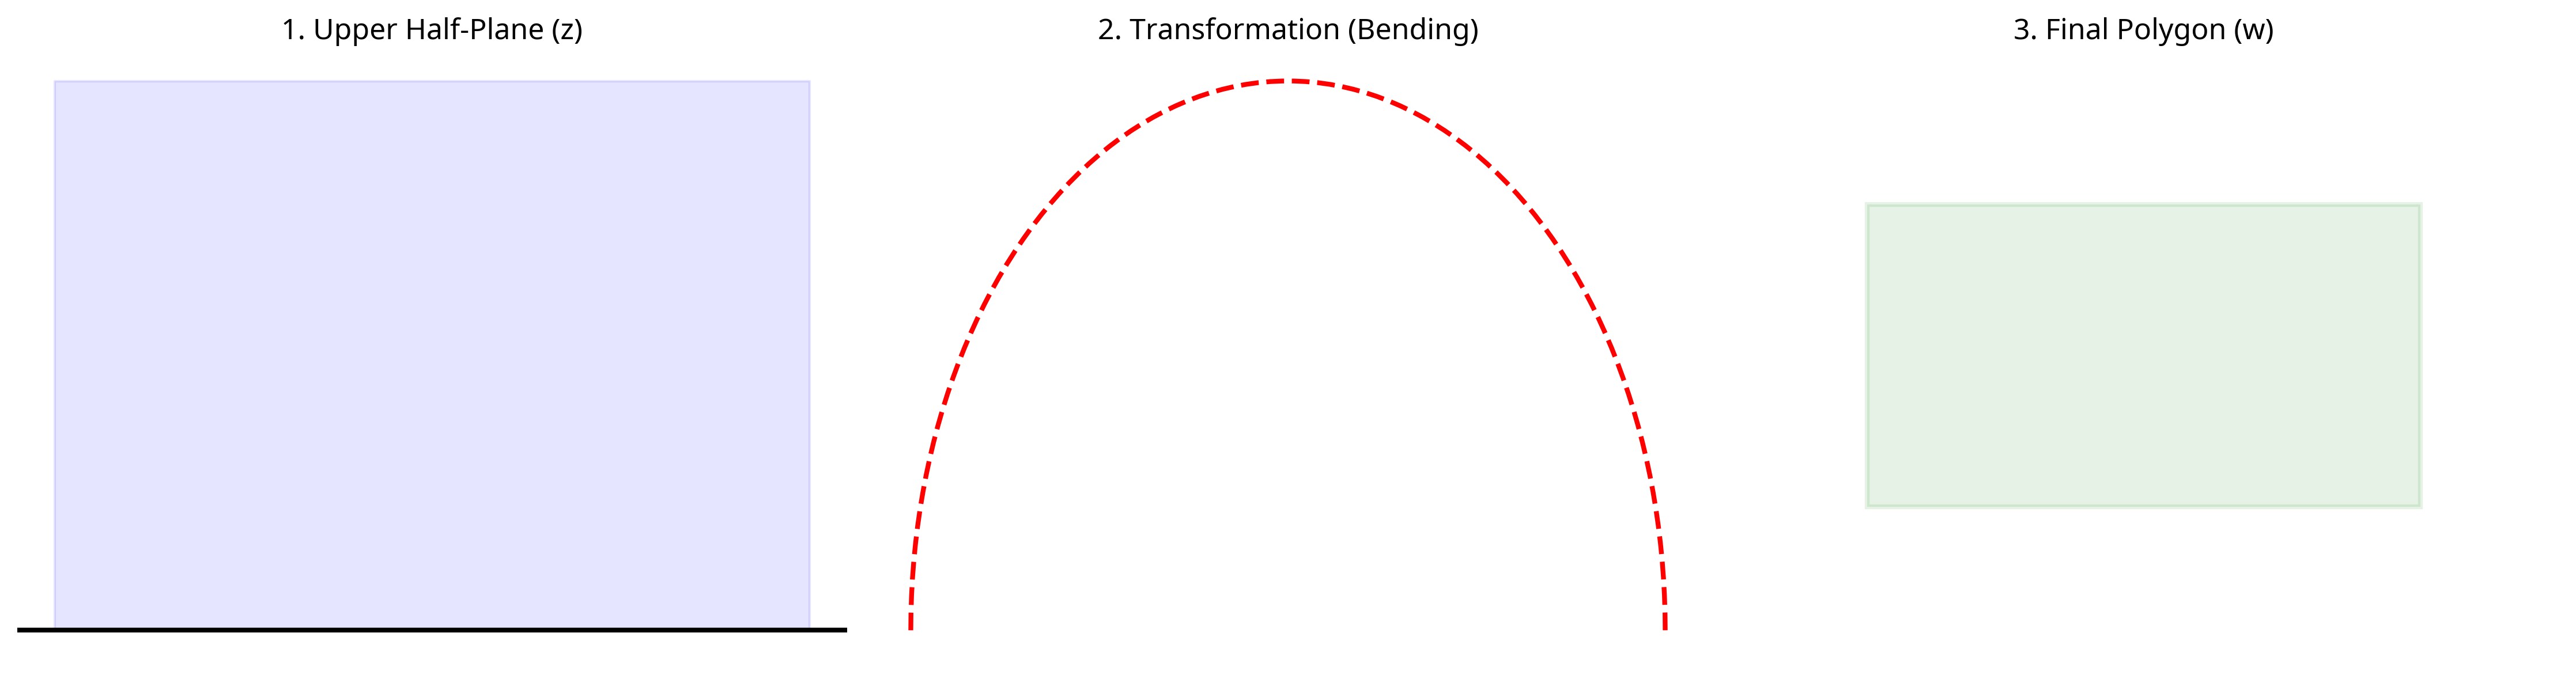
\includegraphics[width=0.9\textwidth]{diagrams/sc_process.png}
    \caption{The three-stage process of an SC transformation: 1. Starting with the half-plane. 2. Applying the bending transformation. 3. Arriving at the final polygonal domain.}
    \label{fig:sc_step}
\end{figure}

\begin{figure}[H]
    \centering
    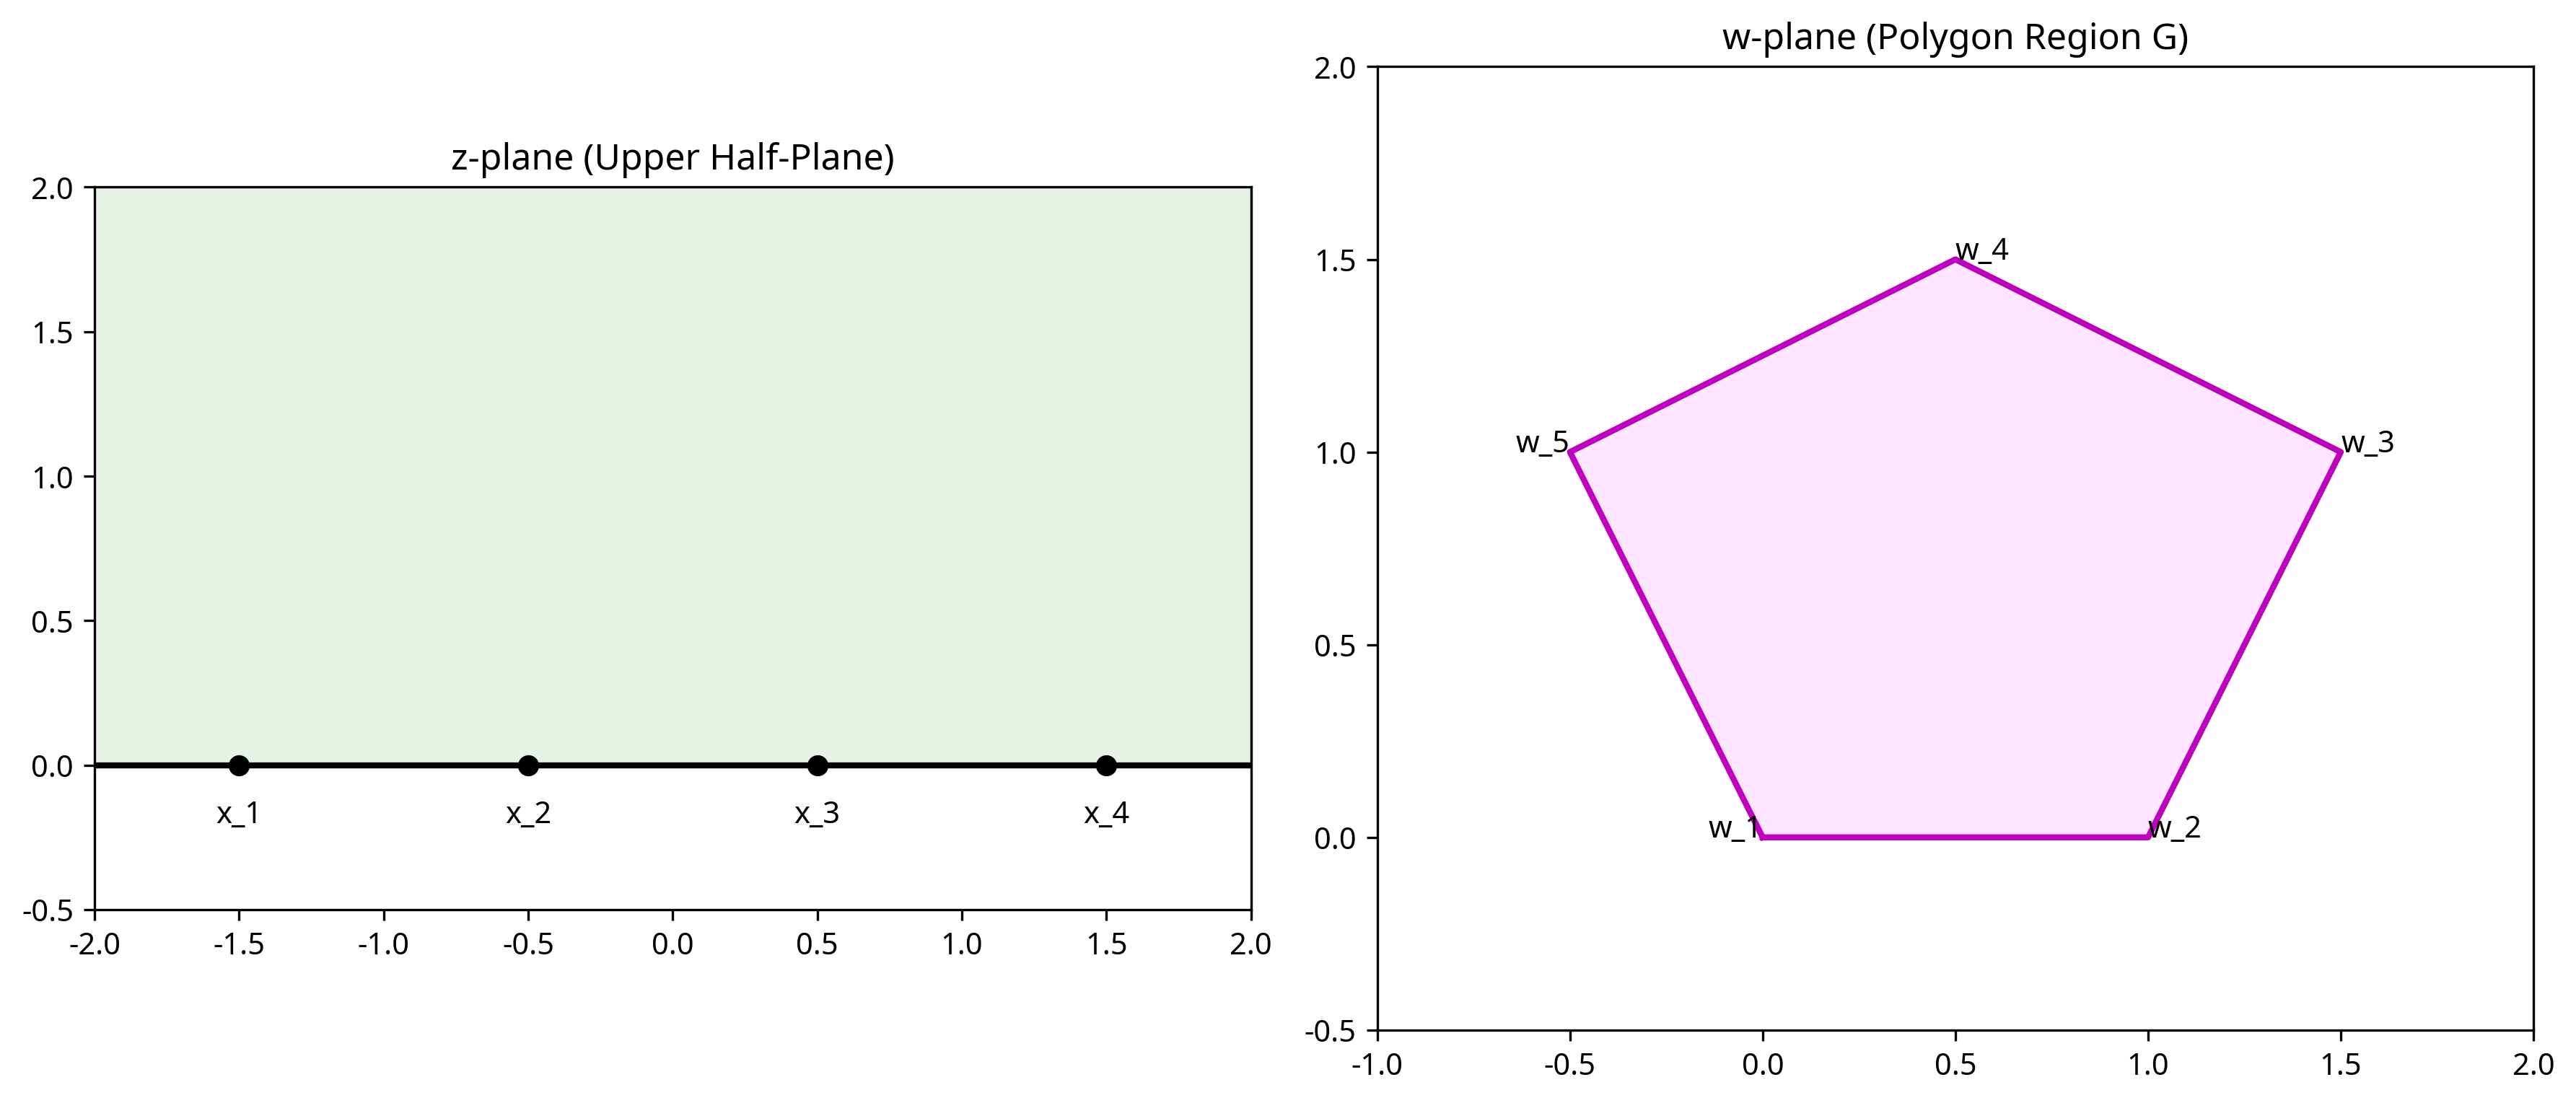
\includegraphics[width=0.8\textwidth]{diagrams/polygon_mapping.png}
    \caption{Conformal mapping from the upper half-plane (z-plane) to a polygonal region (w-plane). The pre-vertices $x_i$ on the real axis correspond to the vertices $w_i$ of the polygon.}
    \label{fig:polygon_mapping}
\end{figure}

\section{Newton's Method for Quadrilateral Mapping}

Solving the system of non-linear equations for the parameters of the Schwarz-Christoffel transformation often requires numerical methods. Newton's method is a widely used iterative technique for finding successively better approximations to the roots (or zeroes) of a real-valued function. In the context of conformal mapping, it is applied to determine the pre-vertices $x_i$ that define the polygonal region. For mapping the upper half-plane onto a quadrilateral, the problem reduces to solving a single non-linear equation $F(k) = 0$, where $k$ is a parameter related to the pre-vertices.

The iterative process of Newton's method involves calculating corrections based on the function's value and its derivative at the current approximation. The general form for the first correction $\delta^{(1)}$ is given by:

\begin{equation}
    \impformula{\delta^{(1)} = -\frac{F(k_0)}{F'(k_0)}} \label{eq:newton_correction}
\end{equation}

where $k_0$ is the initial guess. Subsequent approximations are then found by $k_{n+1} = k_n + \delta^{(n)}$. The convergence properties of Newton's method are crucial, and the text discusses various cases based on the initial guess and the behavior of $F(k)$ and its derivatives.

\begin{figure}[H]
    \centering
    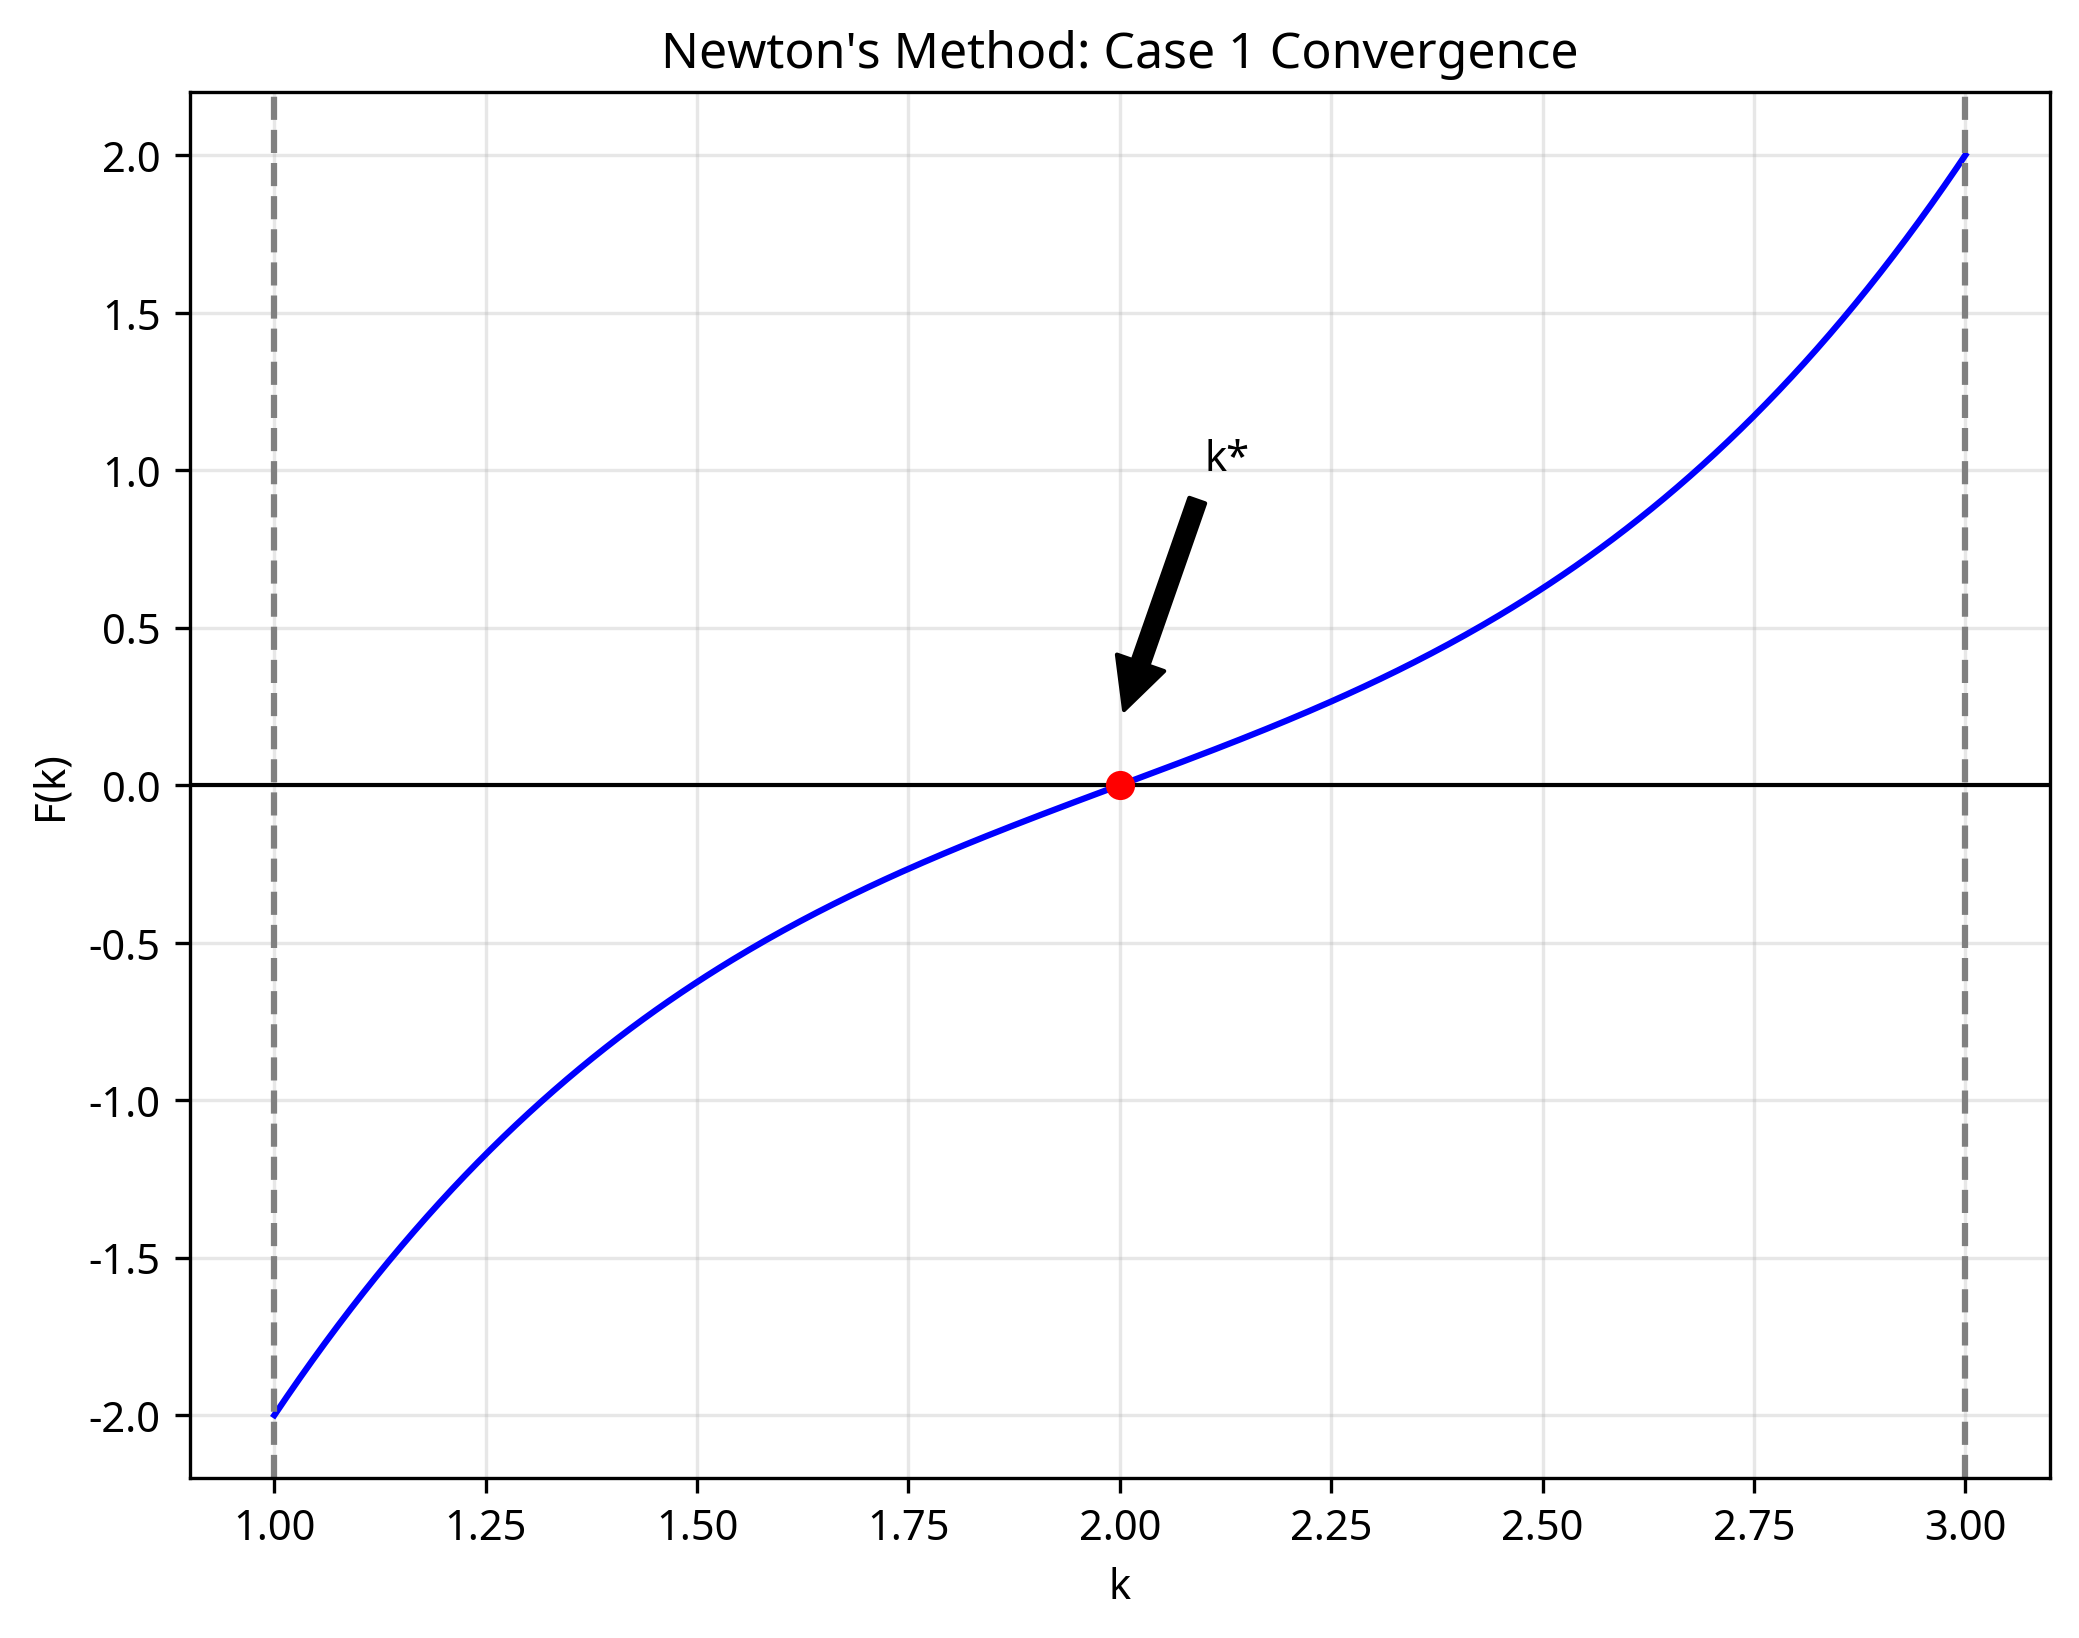
\includegraphics[width=0.7\textwidth]{diagrams/newton_convergence.png}
    \caption{Illustration of Newton's method convergence (Case 1). The function $F(k)$ is shown, and the iterative process converges to the root $k^*$.}
    \label{fig:newton_convergence}
\end{figure}

\section{Numerical Computations and Specific Cases}

This section delves into specific numerical examples and cases where Schwarz-Christoffel integrals are evaluated. The reference provides examples such as determining constants for a trapezoidal mapping and the transformation for a unit disk. For instance, the integral for a specific case might be expressed as:

\begin{equation}
    \impformula{I_4(k) = \int_0^1 (1 + 3t)^{-\alpha_1}(1 + t)^{-\alpha_2}(1 + (2-k)t)^{-\alpha_3}(1-t)^{-\alpha_4} dt + \int_0^1 (1-t)^{-\alpha_1}(1 + t)^{-\alpha_2}(1 + kt)^{-\alpha_3}(1 + 3t)^{-\alpha_4} dt} \label{eq:I4_integral}
\end{equation}

These integrals often require careful numerical evaluation due to singularities. The text details how such integrals are set up and solved iteratively, for example, to find a parameter $k$ such that a ratio of integrals is satisfied.

\begin{figure}[H]
    \centering
    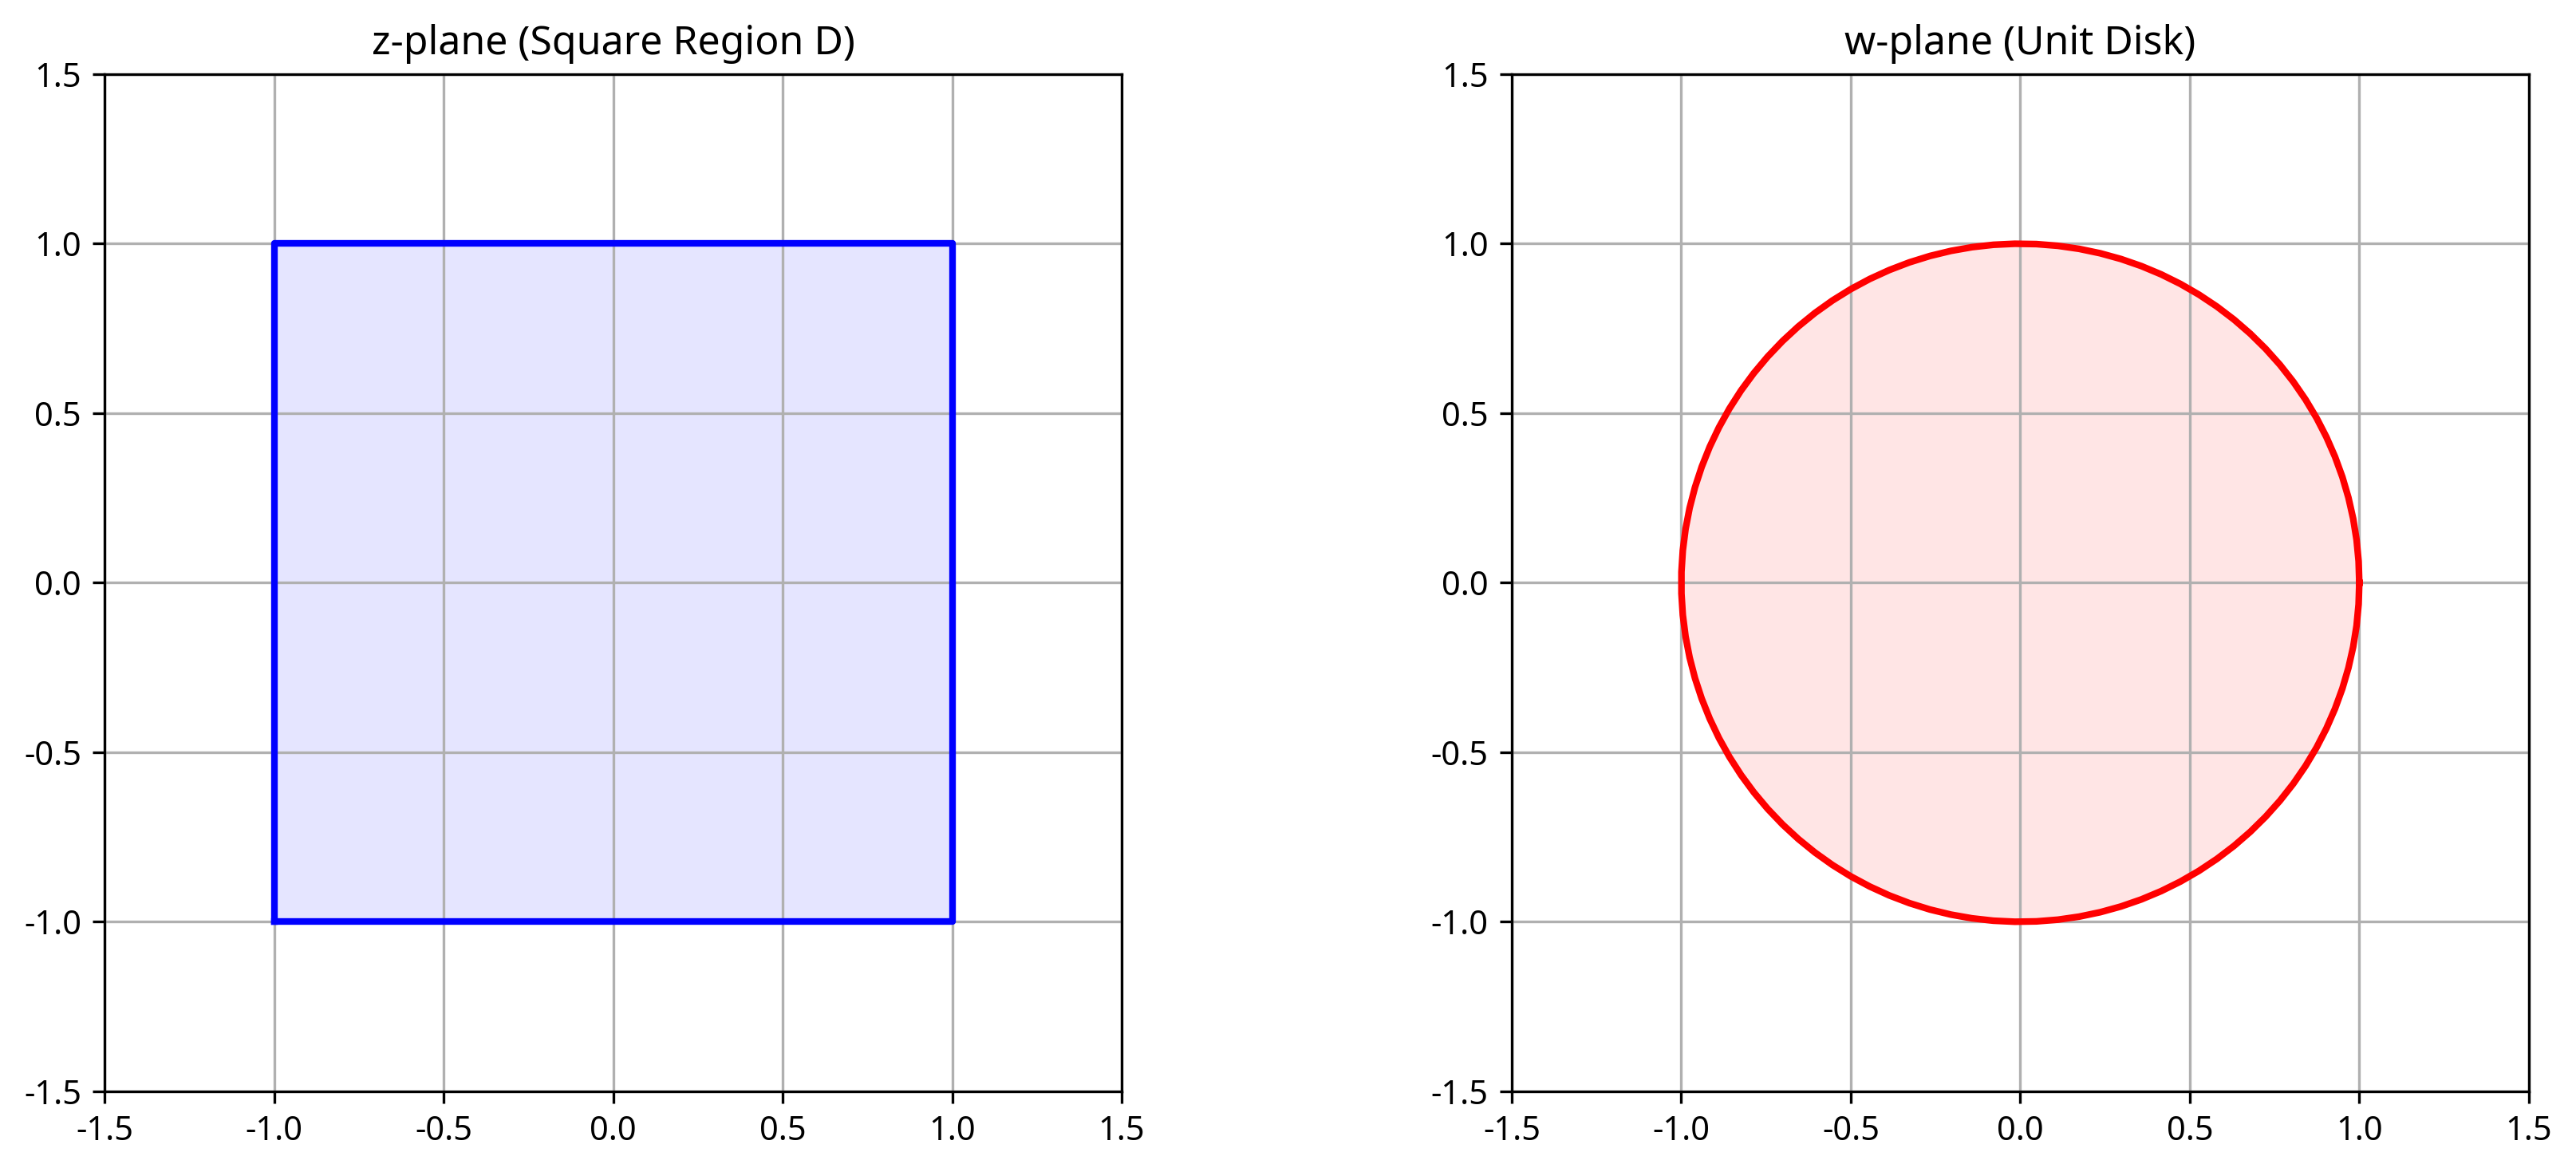
\includegraphics[width=0.7\textwidth]{diagrams/square_to_circle.png}
    \caption{Conformal mapping of a square region in the z-plane onto a unit disk in the w-plane, illustrating a common application of Schwarz-Christoffel transformations.}
    \label{fig:square_to_circle}
\end{figure}

\section{Removal of Singularities}

The integrands in Schwarz-Christoffel formulas often contain singularities at the pre-vertices, making direct numerical integration challenging. Two analytical methods are commonly employed to remove these singularities, thereby facilitating more accurate numerical computations.

\imppoint{Method 1 involves rewriting the integrand by factoring out the singular terms and expressing the remaining part in a form that is bounded or goes to zero at the singularity.} For an exponent $\alpha_1 > 0$, the integrand can be manipulated to isolate the singular behavior, often leading to incomplete beta functions upon integration.

\imppoint{Method 2 utilizes a transformation of variables to eliminate the singularity.} For example, if a singularity exists at $\zeta = x_1$, a transformation like $z_1 = (z - x_1)^{1-\alpha_1}$ can be applied. This transforms the half-plane onto an angular sector, effectively regularizing the integral.

\section{Trefethen's Method for Schwarz-Christoffel Transformation}

Trefethen's method offers an alternative approach to the Schwarz-Christoffel transformation, focusing on mapping a polygon in the z-plane onto the unit disk in the w-plane, rather than the upper half-plane. This method is particularly advantageous for its numerical stability and efficiency. The mapping function is expressed as:

\begin{equation}
    \impformula{w = f(z) = w_c + C \int_0^z \prod_{k=1}^N \left(\frac{z'}{z' - z_k}\right)^{-\alpha_k} dz'} \label{eq:Trefethen_formula}
\end{equation}

where $z_k$ are the pre-vertices on the unit circle, and $w_c$ and $C$ are accessory parameters. The determination of these accessory parameters is a key aspect of the parameter problem in this context. Trefethen's method formulates this as a constrained nonlinear system, which is then solved iteratively, often using Newton's method combined with techniques like Gauss-Jacobi quadrature for integral evaluation. \imppoint{A crucial aspect is the careful spacing of pre-vertices around the unit circle to maintain numerical accuracy, adhering to the principle that no singularity should lie too close to an integration interval.}

\chapter{Physical Applications of Conformal Mapping}

Conformal mapping is a workhorse for solving Laplace's equation $\nabla^2 \Phi = 0$ in complex geometries. This chapter illustrates how the theoretical transformations are applied to real-world physics problems.

\section{Electrostatics and Potential Theory}
In electrostatics, the potential $\Phi$ satisfies Laplace's equation. If we can map a complex boundary (like a notched electrode) to a flat plane, the potential becomes a simple linear function of the coordinates.

\begin{figure}[H]
    \centering
    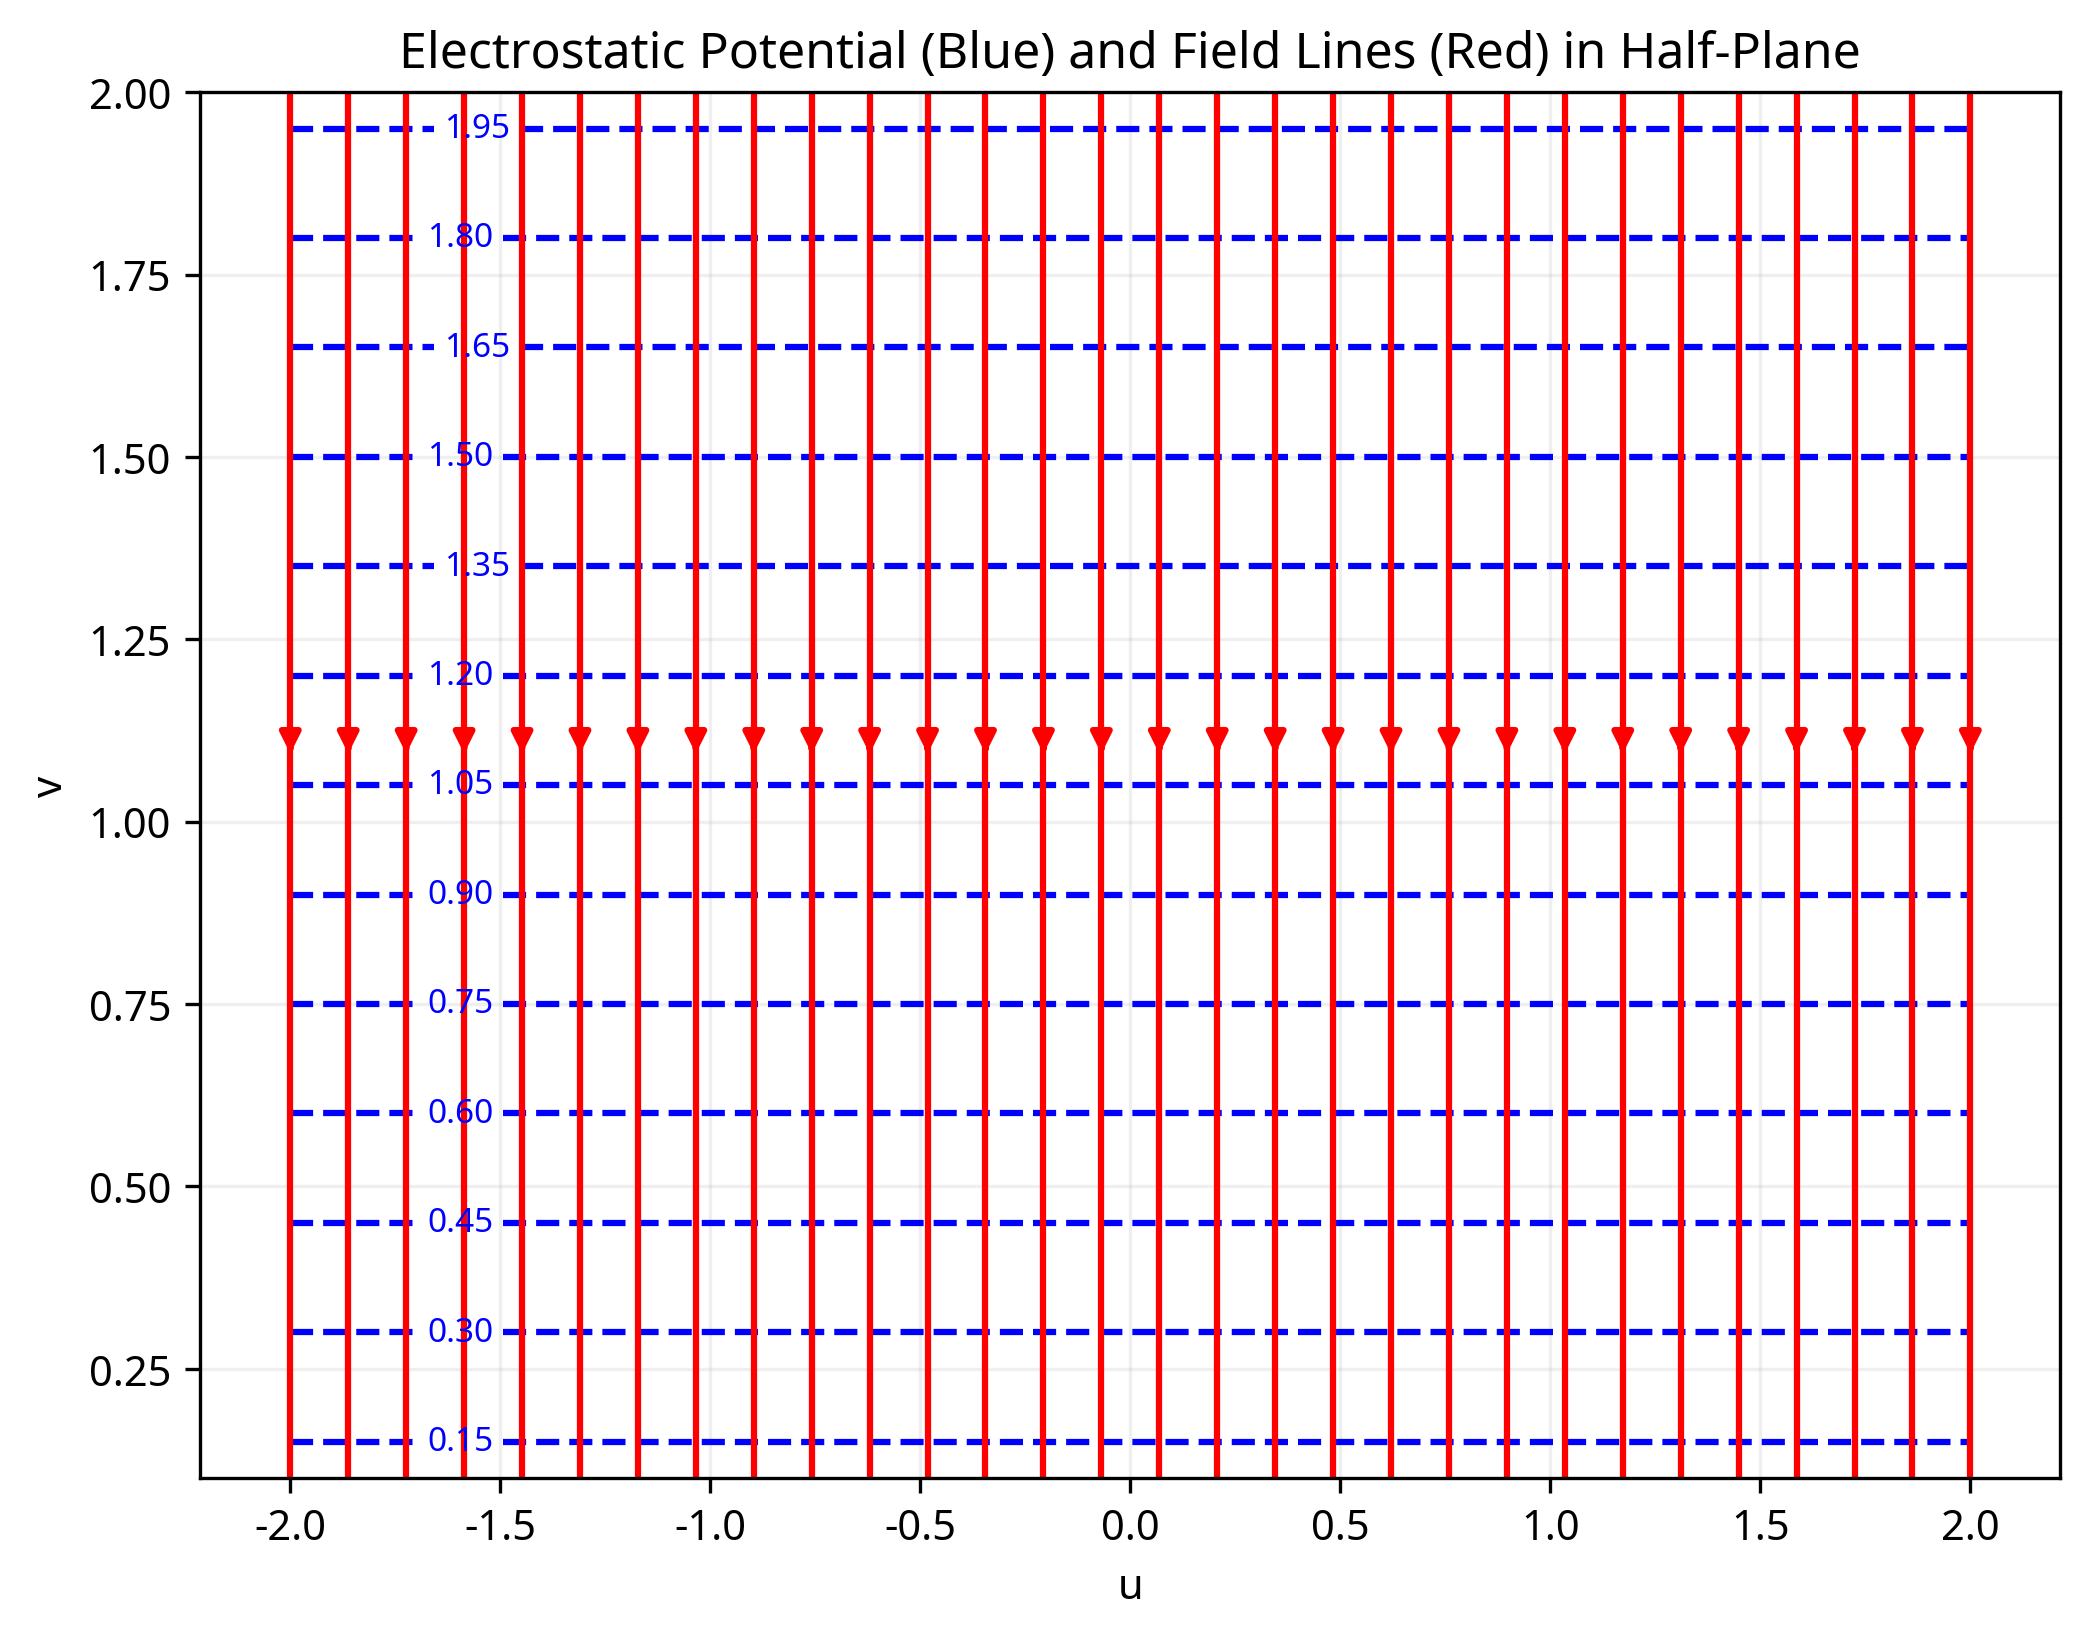
\includegraphics[width=0.7\textwidth]{diagrams/electrostatic_half_plane.png}
    \caption{Equipotential lines (dashed) and field lines (solid) in a simplified half-plane domain. Conformal maps allow us to "wrap" this simple solution around complex objects.}
    \label{fig:electro}
\end{figure}

\section{Fluid Dynamics and Streamlines}
For irrotational, incompressible fluid flow, the velocity potential and stream function form a complex potential $F(z) = \phi + i\psi$. The curves $\psi = \text{constant}$ are the streamlines of the flow. By solving for flow around a circle and then applying a transform, engineers can predict the pressure distribution over complex shapes.

\begin{figure}[H]
    \centering
    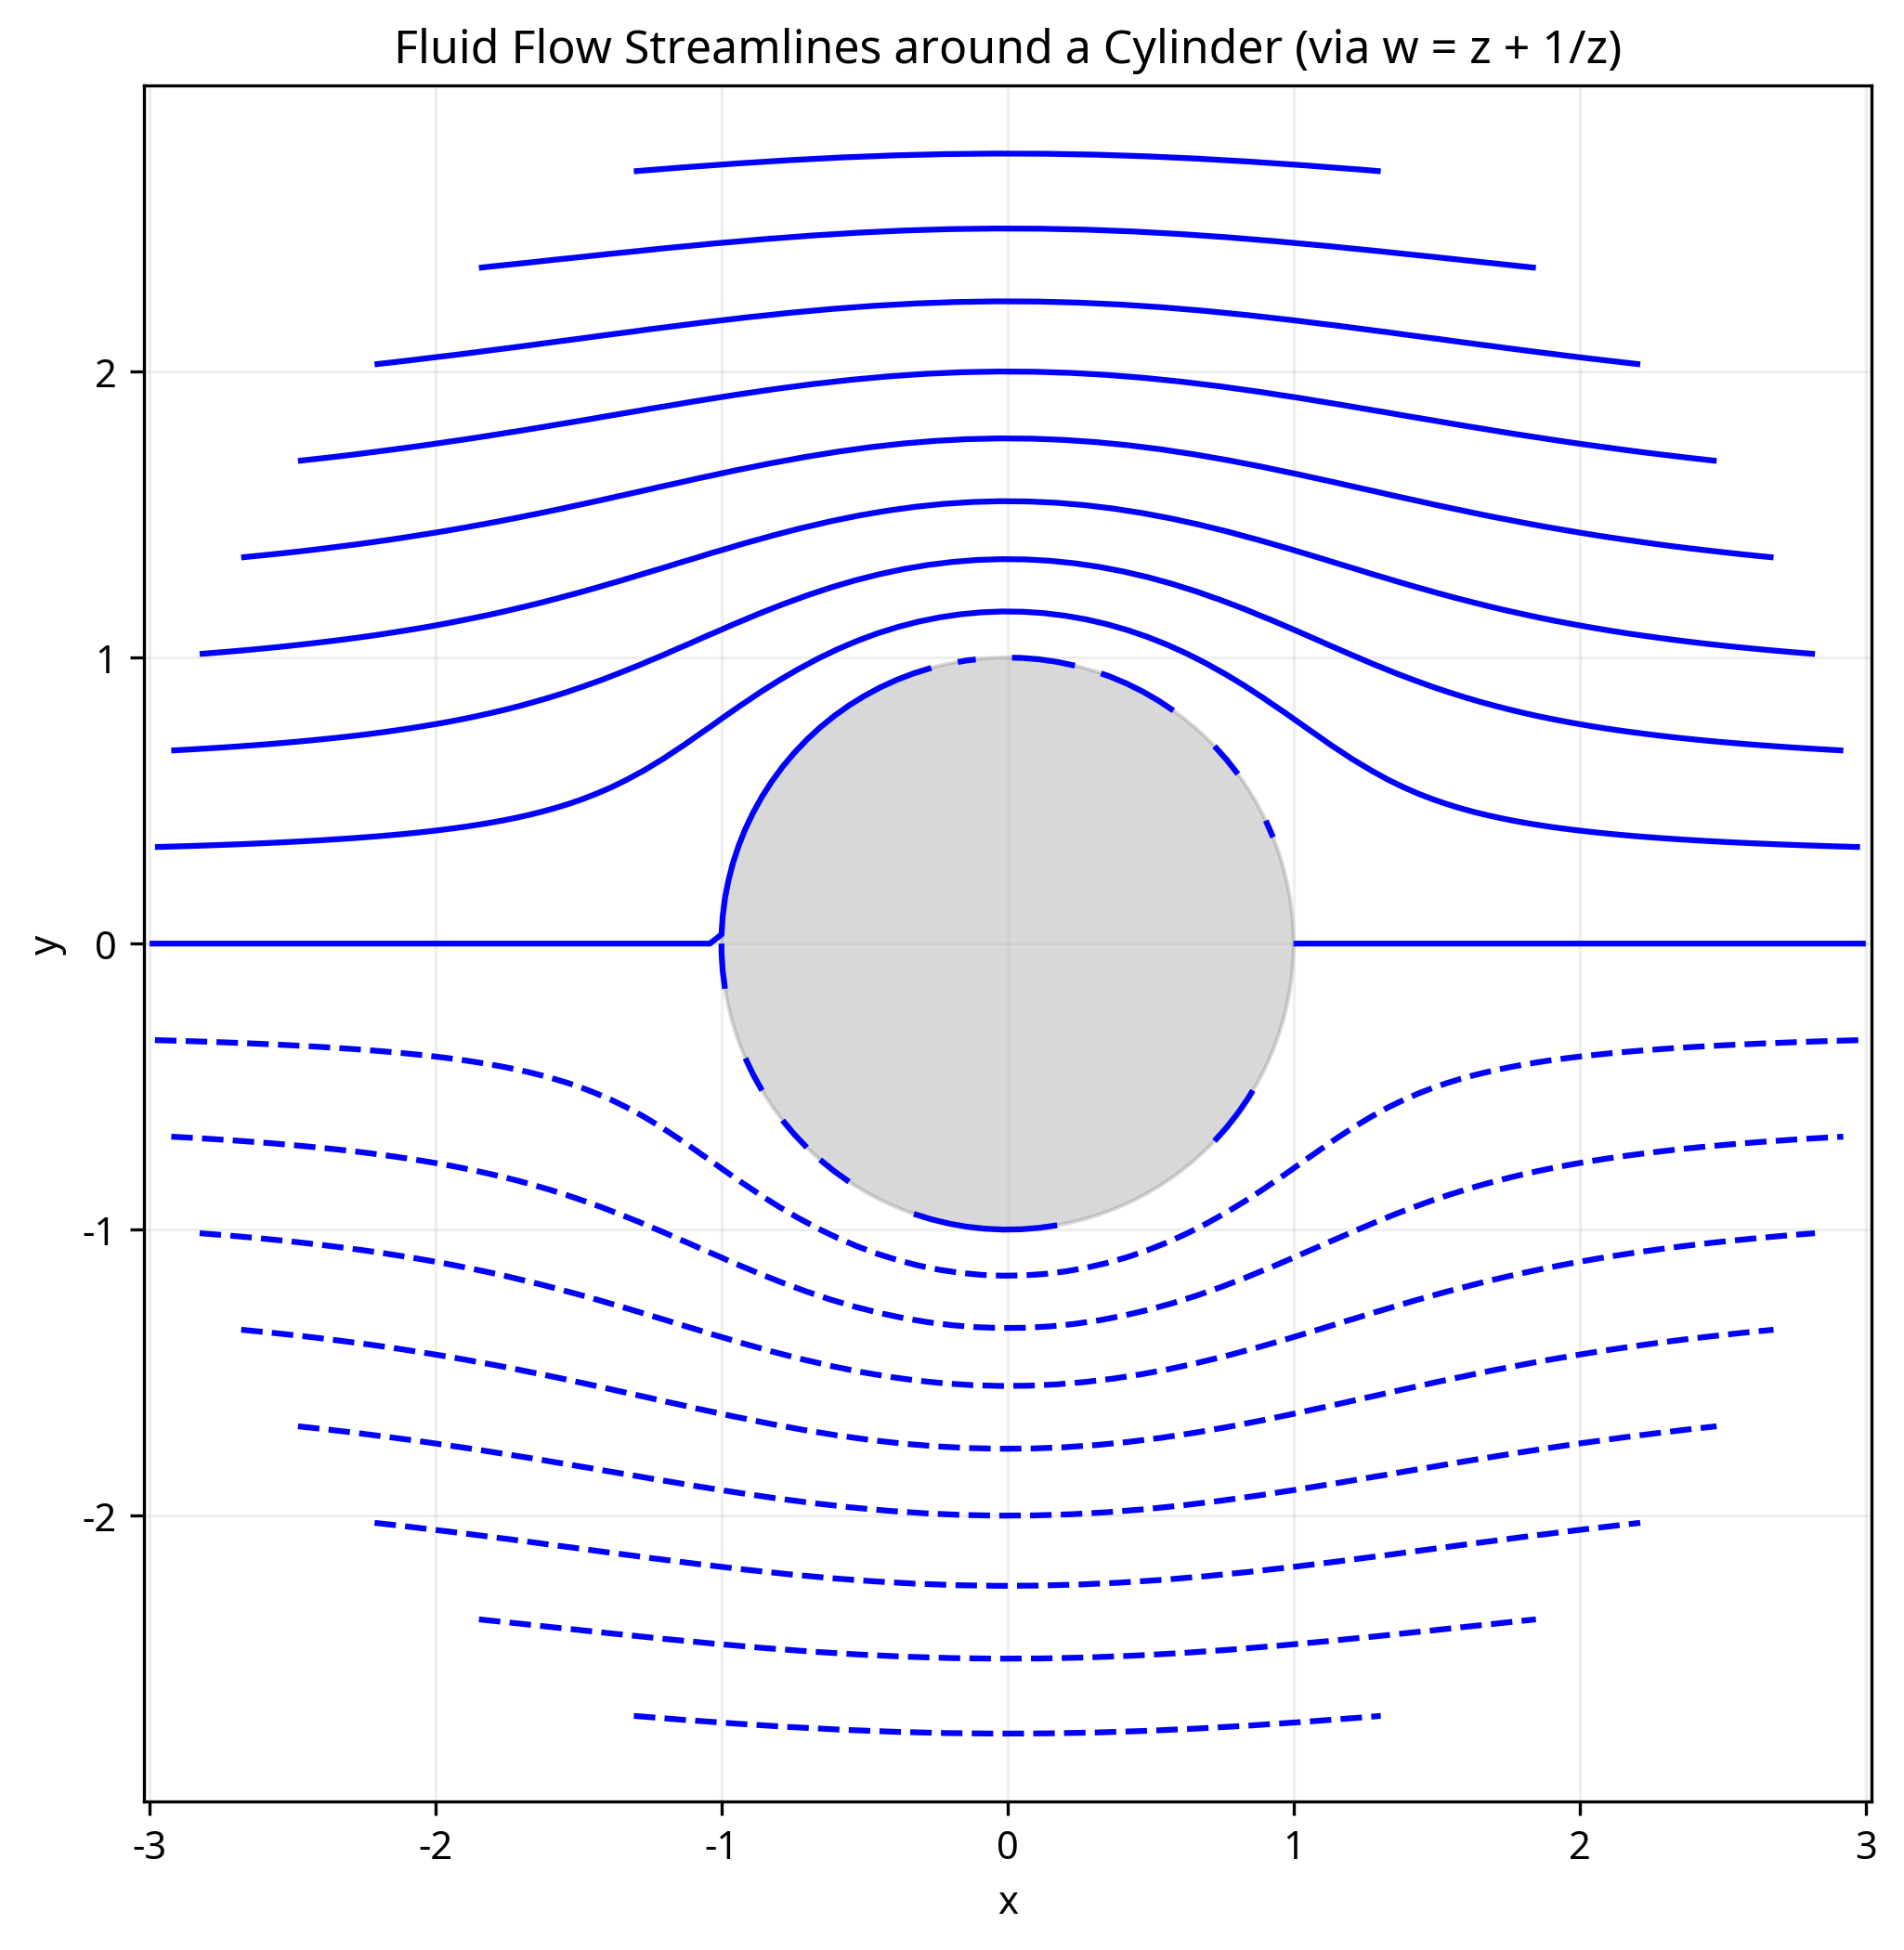
\includegraphics[width=0.7\textwidth]{diagrams/fluid_flow_cylinder.png}
    \caption{Streamlines of fluid flow around a cylinder. This pattern is derived by mapping a uniform flow in the $w$-plane back to the $z$-plane using the Joukowsky transform or similar mappings.}
    \label{fig:fluid}
\end{figure}

\chapter{Minimum Area Problem}

\begin{figure}[H]
    \centering
    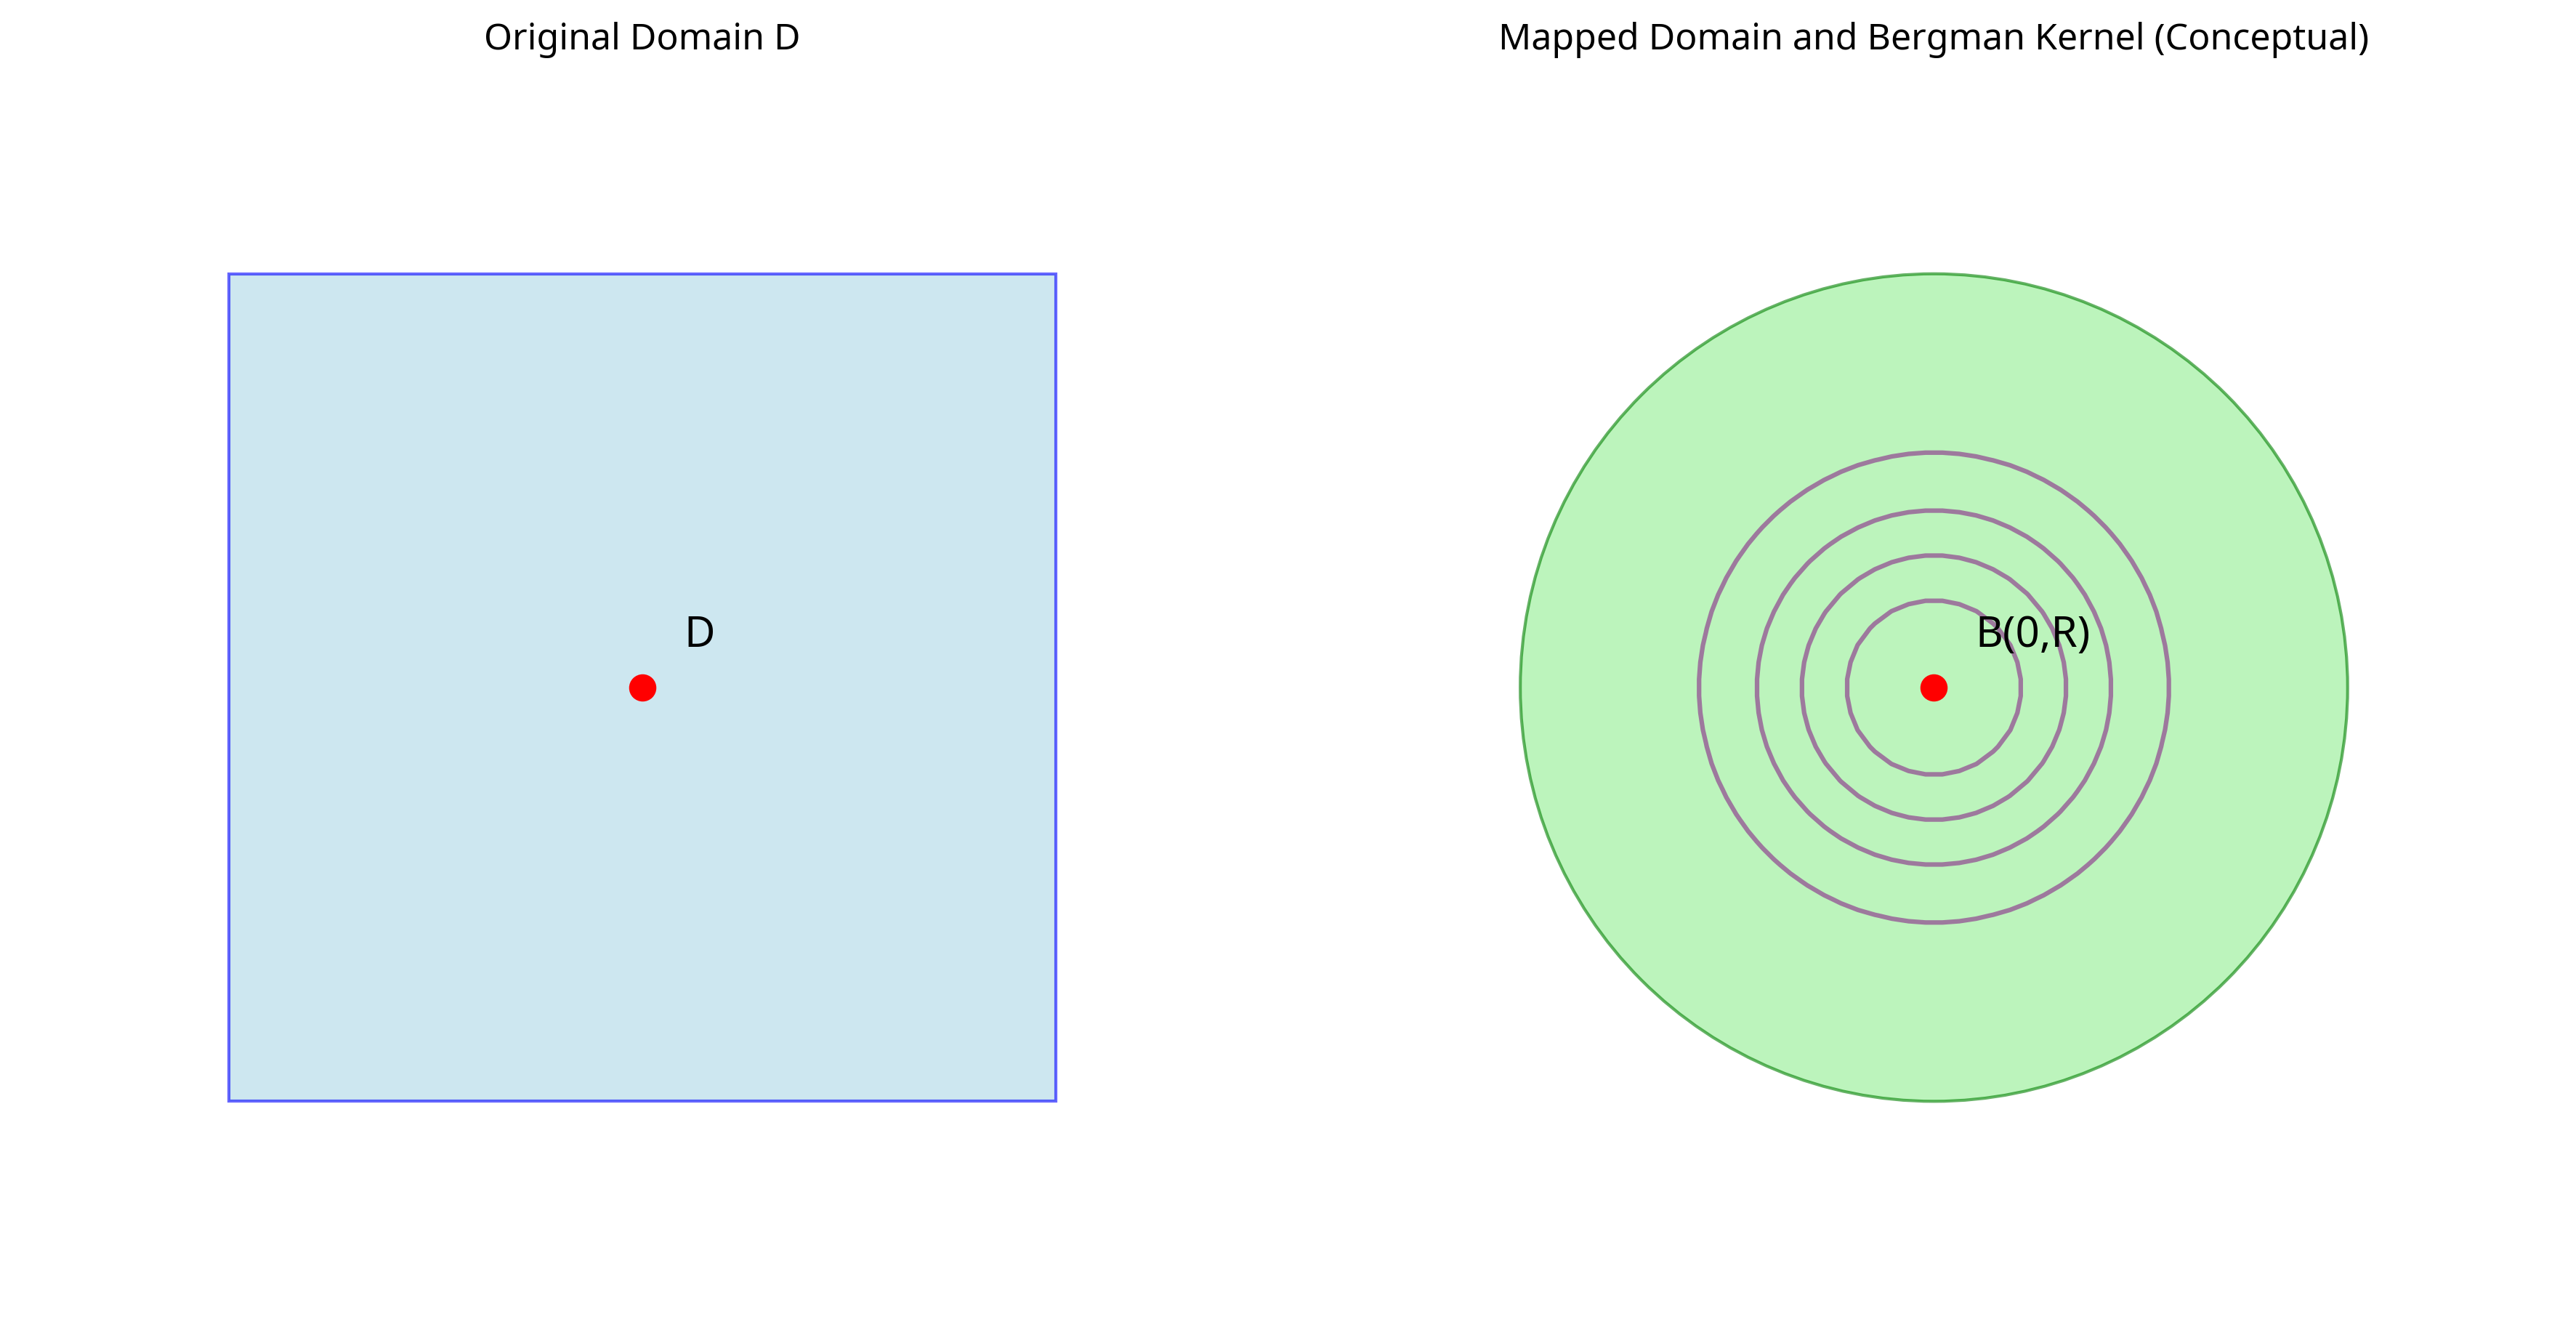
\includegraphics[width=0.8\textwidth]{diagrams/bergman_kernel_concept.png}
    \caption{Conceptual visualization of the Bergman Kernel. The original domain D is mapped to a disk, and the kernel function highlights the point of interest, illustrating its reproductive property.}
    \label{fig:bergman_kernel_concept}
\end{figure}


This chapter explores extremal problems in conformal mapping, specifically focusing on the minimum area problem, also known as Problem I or the Bieberbach minimizing principle. This problem seeks to find a conformal mapping that minimizes the area of the mapped region under certain conditions.

\section{Gaier's Variational Method and Bieberbach Principle}

Gaier's variational method is a powerful technique used to solve extremal problems in conformal mapping. The minimum area problem is concerned with mapping a simply connected region $D$ onto a disk $B(0,R)$ in the w-plane such that the area of the image is minimized. The mapping function $f(z)$ is regular in $D$ and satisfies certain normalization conditions, such as $f(a) = 1$ for some $a \in D$. The integral to be minimized is given by:

\begin{equation}
    \impformula{I = \iint_D |f'(z)|^2 dS_z} \label{eq:min_area_integral}
\end{equation}

where $dS_z$ is the area element in the z-plane. The Riemann mapping theorem guarantees the existence and uniqueness of the solution to this extremal problem, stating that the minimum area is $\pi R^2$.

\section{Bergman Kernel}

The Bergman kernel function plays a significant role in the theory of conformal mapping, particularly in relation to the minimum area problem. It provides a way to characterize the minimal mapping function. The Bergman kernel $K(z,a)$ is defined in terms of the minimal function $f_0(z)$ as:

\begin{equation}
    \impformula{K(z,a) = \frac{f_0(z)}{\|f_0\|^2}} \label{eq:bergman_kernel_def}
\end{equation}

where $\|f_0\|^2 = \iint_D |f_0(z)|^2 dS_z$. A key property of the Bergman kernel is that for every function $f \in L^2(D)$, the integral $\iint_D K(z,a)f(z)dS_z = f(a)$. This property highlights the reproductive nature of the kernel. The minimal function $f_0(z)$ itself can be expressed in terms of the Bergman kernel as $f_0(z) = K(z,a)/K(a,a)$.

\section{Numerical Methods: Ritz Method}

The Ritz method is a powerful numerical technique used to find approximate solutions to extremal problems, including the minimum area problem. It involves approximating the minimal function by a polynomial. The method considers an arbitrary system of linearly independent functions $u_k(z)$ that are regular in $D$. The goal is to choose coefficients $c_k$ for a polynomial $\varphi_n(z) = \sum_{k=0}^n c_k u_k(z)$ such that the integral $I(\varphi_n) = \iint_D |\varphi_n'(z)|^2 dS_z$ is minimized, subject to certain conditions like $\varphi_n(0) = 1$.

This minimization leads to a system of linear equations that determine the coefficients $c_k$. The coefficients $A_{kj}$ in this system are derived from integrals involving the basis functions:

\begin{equation}
    \impformula{A_{kj} = \iint_D z^k \overline{z^j} dS_z} \label{eq:ritz_coefficients}
\end{equation}

for a specific choice of basis functions $u_k(z) = z^k$. The uniqueness of the solution and the completeness of the polynomial system are important theoretical aspects.

\section{Bergman Kernel Method}

Similar to the Ritz method, the Bergman kernel method provides a numerical approach to approximate the mapping function for the minimum area problem. This method leverages the Fourier series expansion of the Bergman kernel. If $\{\varphi_j^*(z)\}$ is a complete orthonormal set of $L^2(D)$, then the Bergman kernel $K(z,0)$ can be expanded as:

\begin{equation}
    \impformula{K(z,0) = \sum_{j=1}^\infty \varphi_j^*(0) \varphi_j^*(z)} \label{eq:bergman_series}
\end{equation}

This series converges in the mean of $L^2(D)$. By using this expansion and the relationship between the mapping function and the Bergman kernel, an approximate mapping function can be obtained. The process often involves orthonormalizing a set of basis functions using the Gram-Schmidt process.

\chapter{Minimum Boundary Problem}

\begin{figure}[H]
    \centering
    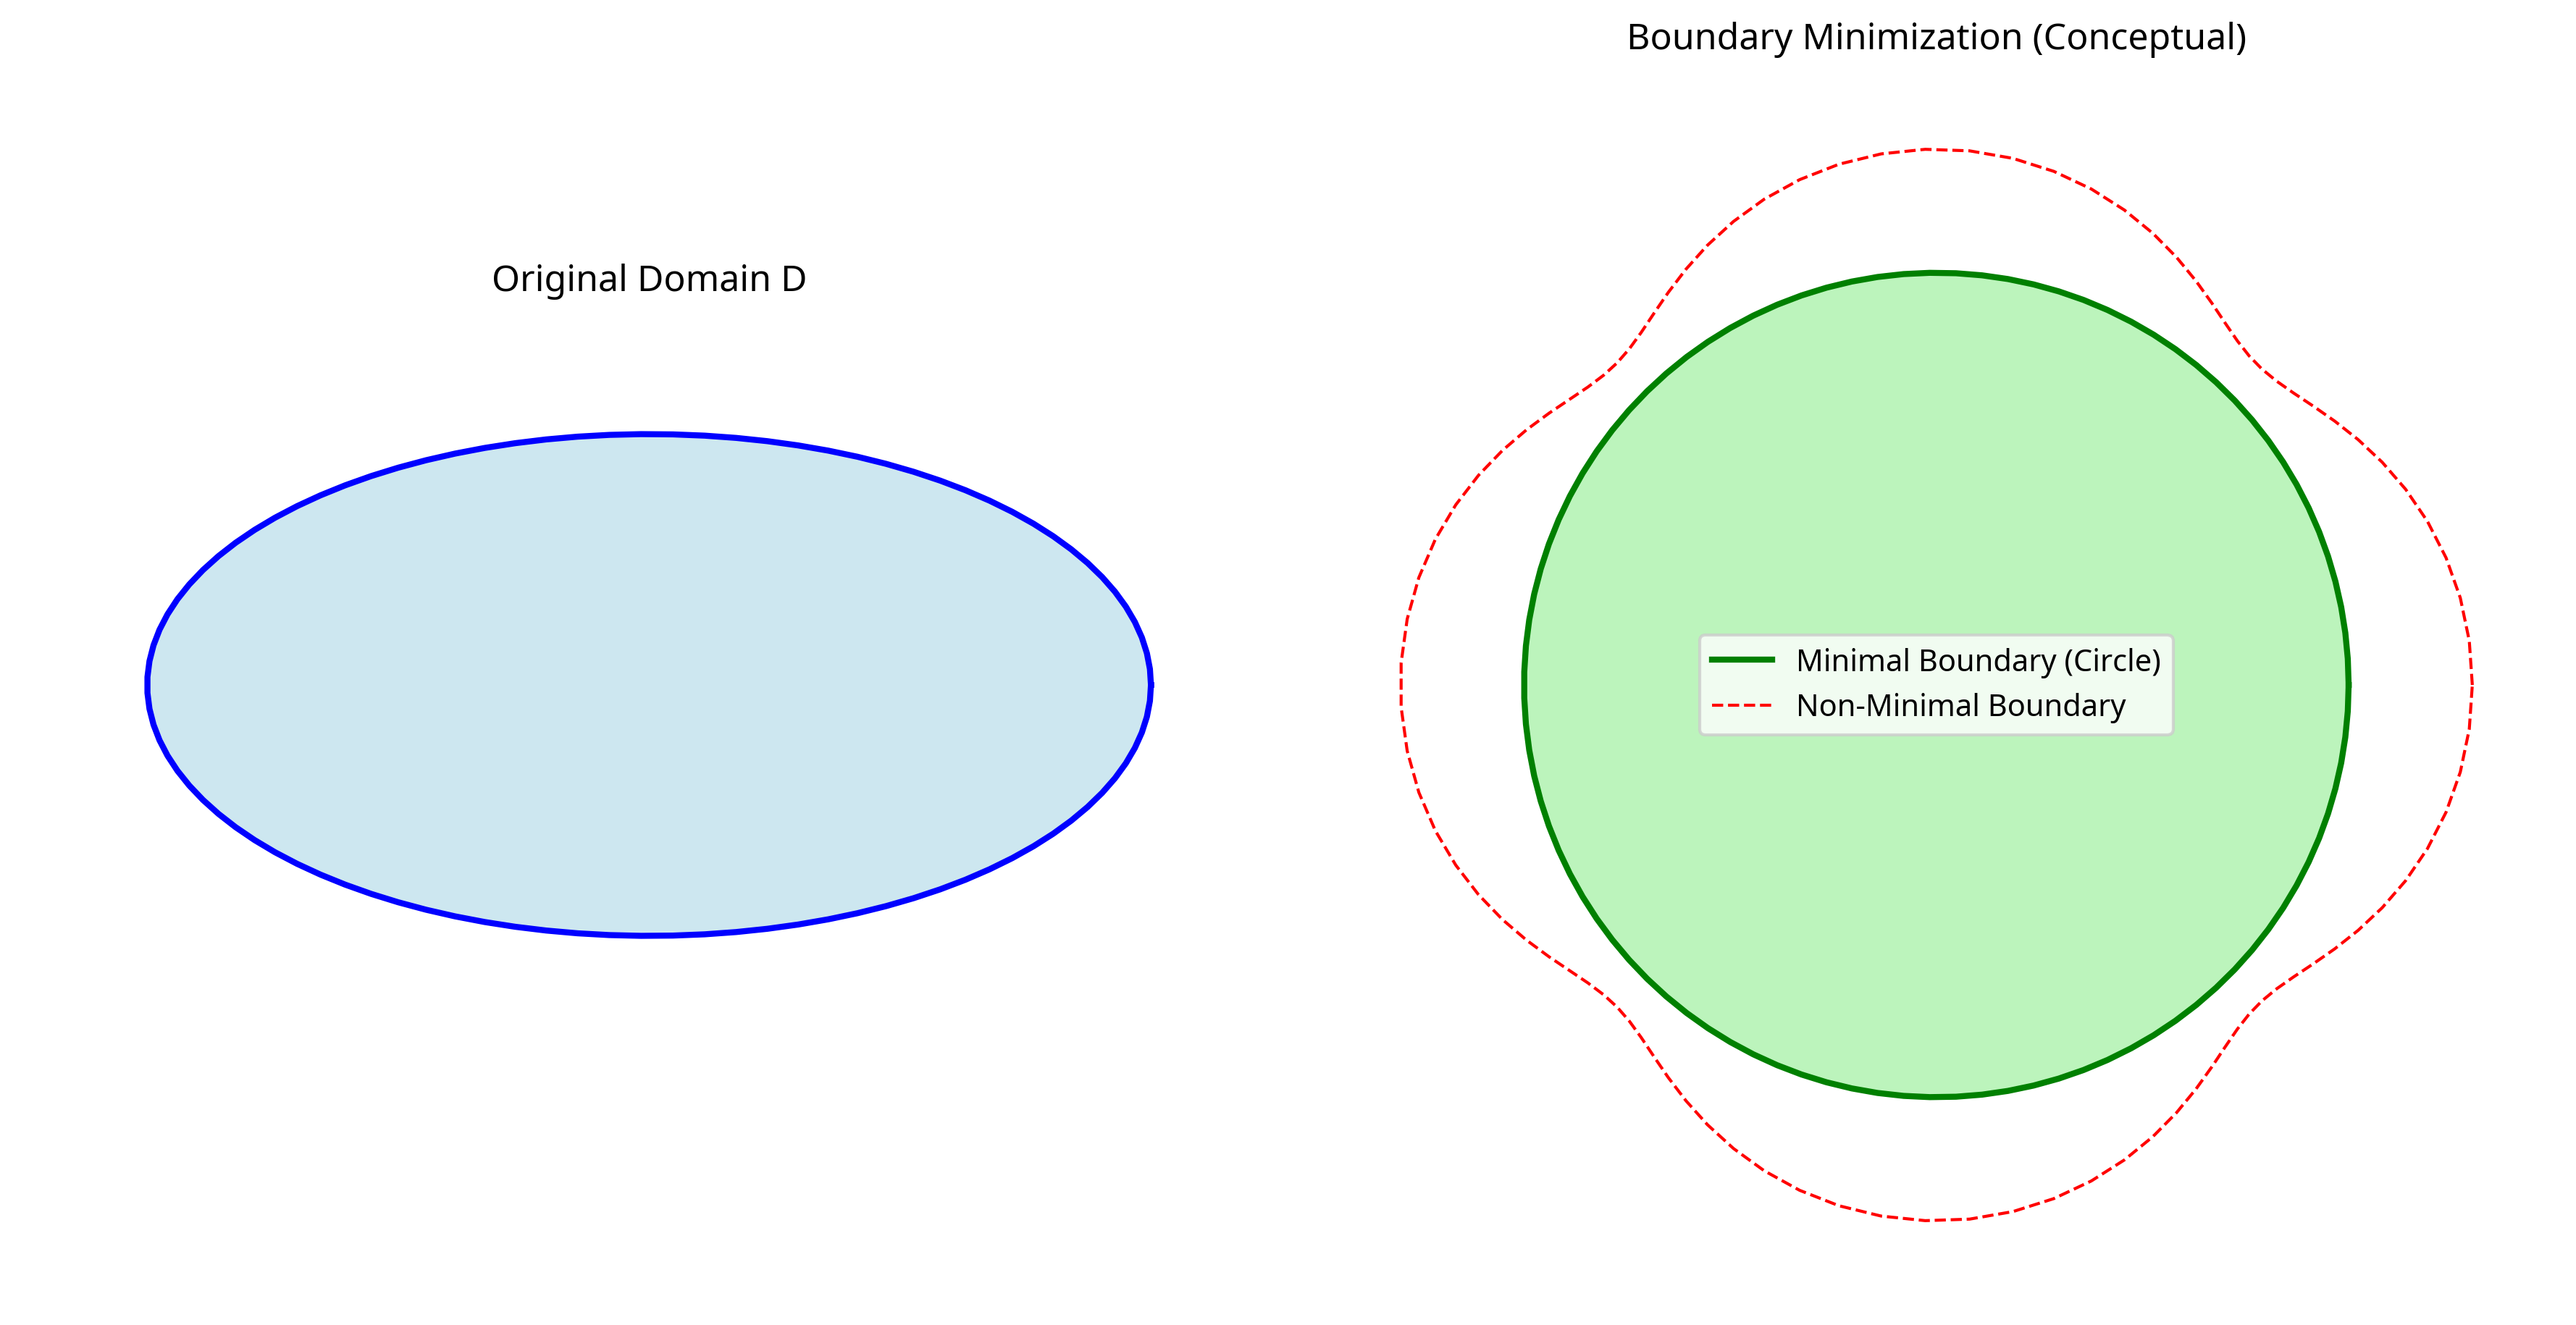
\includegraphics[width=0.8\textwidth]{diagrams/boundary_minimization_concept.png}
    \caption{Conceptual illustration of boundary minimization. An original domain is mapped to a unit circle, demonstrating how the minimal boundary solution is achieved compared to a non-minimal boundary.}
    \label{fig:boundary_minimization_concept}
\end{figure}


This chapter introduces another extremal problem in conformal mapping: the minimum boundary problem, also known as Problem II or Julia's method. This problem focuses on minimizing the length of the boundary of the mapped region.

\section{Julia's Method and Minimum Boundary Principle}

The minimum boundary problem is concerned with mapping a region $D$ onto a disk $|w| < R$ such that the line integral of the magnitude of the mapping function along the boundary $\Gamma$ of $D$ is minimized. The integral to be minimized is:

\begin{equation}
    \impformula{I = \int_\Gamma |f(z)|^2 ds} \label{eq:min_boundary_integral}
\end{equation}

where $ds$ is the arc length element along the boundary. Similar to the minimum area problem, this problem has a unique solution, and the minimum value is $2\pi R$. This principle is also known as minimizing the image boundary.

\section{Szego Kernel}

Analogous to the Bergman kernel for the minimum area problem, the Szego kernel function $S(z,a)$ is introduced for the minimum boundary problem. It characterizes the minimal function $f_0(z)$ for Problem II. The Szego kernel is defined as:

\begin{equation}
    \impformula{S(z,a) = \frac{f_0(z)}{\int_\Gamma |f_0(z)|^2 ds}} \label{eq:szego_kernel_def}
\end{equation}

with properties similar to the Bergman kernel, including a reproductive property: $\int_\Gamma S(z,a)f(z)ds = f(a)$ for any $f \in L^2(\Gamma)$. An important relationship exists between the Bergman and Szego kernels:

\begin{equation}
    \impformula{K(z,a) = 4\pi [S(z,a)]^2} \label{eq:bergman_szego_relation}
\end{equation}

This relation allows for the evaluation of one kernel if the other is known.

\section{Numerical Methods: Ritz Method for Problem II}

The Ritz method can also be applied to solve the minimum boundary problem numerically. It involves finding a minimal polynomial $\varphi_n(z)$ of degree $n$ that minimizes the line integral $\int_\Gamma |\varphi_n(z)|^2 ds$, subject to conditions like $\varphi_n(a) = 1$. The coefficients of this polynomial are determined by solving a system of linear equations, where the coefficients $B_{kj}$ are given by:

\begin{equation}
    \impformula{B_{kj} = \int_\Gamma (z-a)^k \overline{(z-a)^j} ds} \label{eq:ritz_coefficients_boundary}
\end{equation}

These equations ensure that the polynomial satisfies orthogonality conditions, leading to a unique minimal polynomial.

\section{S-Condition and Completeness of Polynomials}

The completeness of polynomial systems in the Hilbert space $L^2(\Gamma)$ is a critical theoretical aspect for the convergence of numerical methods like the Ritz method. The S-condition, given by Smirnov, provides a necessary and sufficient condition for the completeness of polynomials. It relates to the behavior of the inverse mapping function $g(w)$ that maps the disk $|w| < R$ onto the region $D$.

\begin{equation}
    \impformula{\log |g'(w)| = \frac{1}{2\pi} \int_0^{2\pi} \frac{R^2 - r^2}{R^2 - 2Rr\cos(\alpha - \theta) + r^2} \log |g'(Re^{i\alpha})| d\alpha} \label{eq:s_condition}
\end{equation}

Regions whose mapping satisfies the S-condition are said to belong to the Smirnov class $S$. This condition ensures that an arbitrary function in $L^2(\Gamma)$ can be represented by a Fourier series that converges uniformly in $D$.

\section{Extremal Problems in Multiply Connected Regions}
While the majority of this report focuses on simply connected regions, the theory of extremal problems extends to multiply connected regions as well. For a region of connectivity $n$, the mapping function is typically more complex, involving the Schottky-Klein prime function. The minimum area and boundary principles still apply, but the kernels must be modified to account for the additional boundary components. This area of research is particularly relevant in modern computational physics for modeling complex perforated materials and multi-electrode systems.

\section{Theoretical Bounds and Error Analysis}
In numerical conformal mapping, it is essential to establish theoretical bounds on the approximation error. For the Ritz method, the error between the true mapping function $f(z)$ and the $n$-th degree polynomial approximation $\varphi_n(z)$ can be bounded by the rate of decay of the Fourier coefficients. \imppoint{As $n$ increases, the approximation converges to the true function at a rate determined by the smoothness of the boundary $\Gamma$.} If the boundary is analytic, the convergence is exponential; if the boundary has corners (as in polygons), the convergence is algebraic, requiring specialized techniques like the Schwarz-Christoffel transformation to maintain high precision.

\chapter{Numerical Parameter Problem}

\begin{figure}[H]
    \centering
    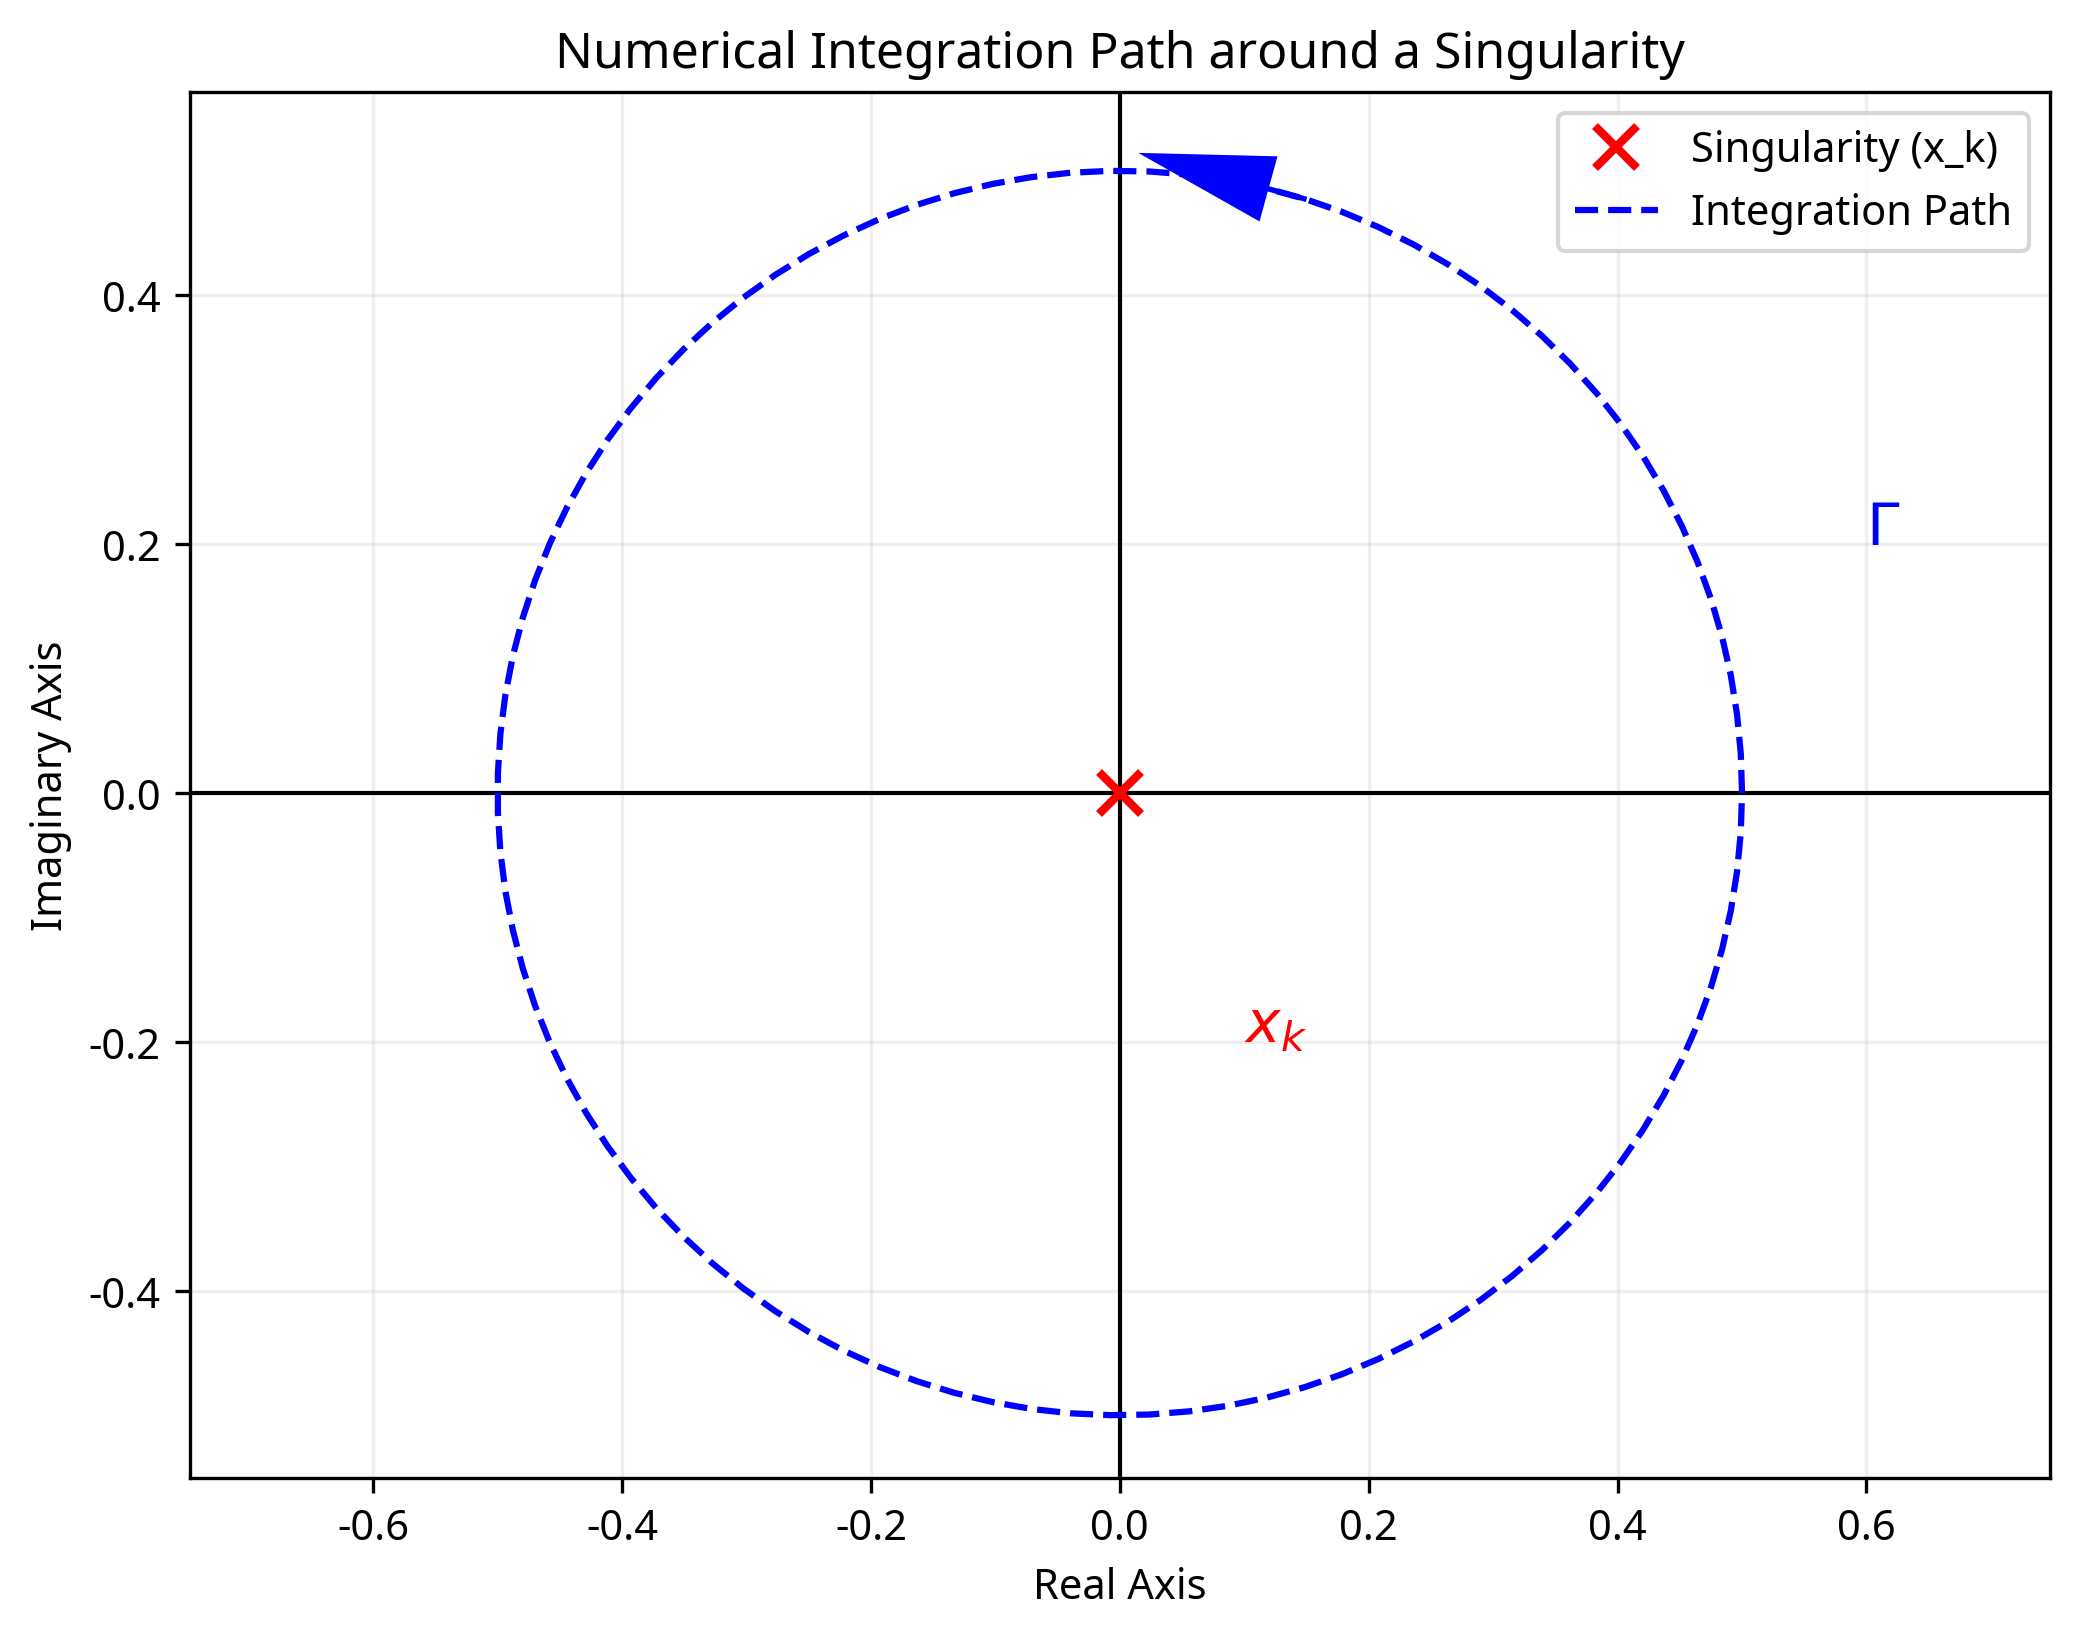
\includegraphics[width=0.8\textwidth]{diagrams/integration_path_singularity.png}
    \caption{Numerical integration path around a singularity. This conceptual diagram shows how the integration contour avoids the singular point $x_k$ on the real axis, crucial for accurate numerical evaluation of Schwarz-Christoffel integrals.}
    \label{fig:integration_path_singularity}
\end{figure}

\begin{figure}[H]
    \centering
    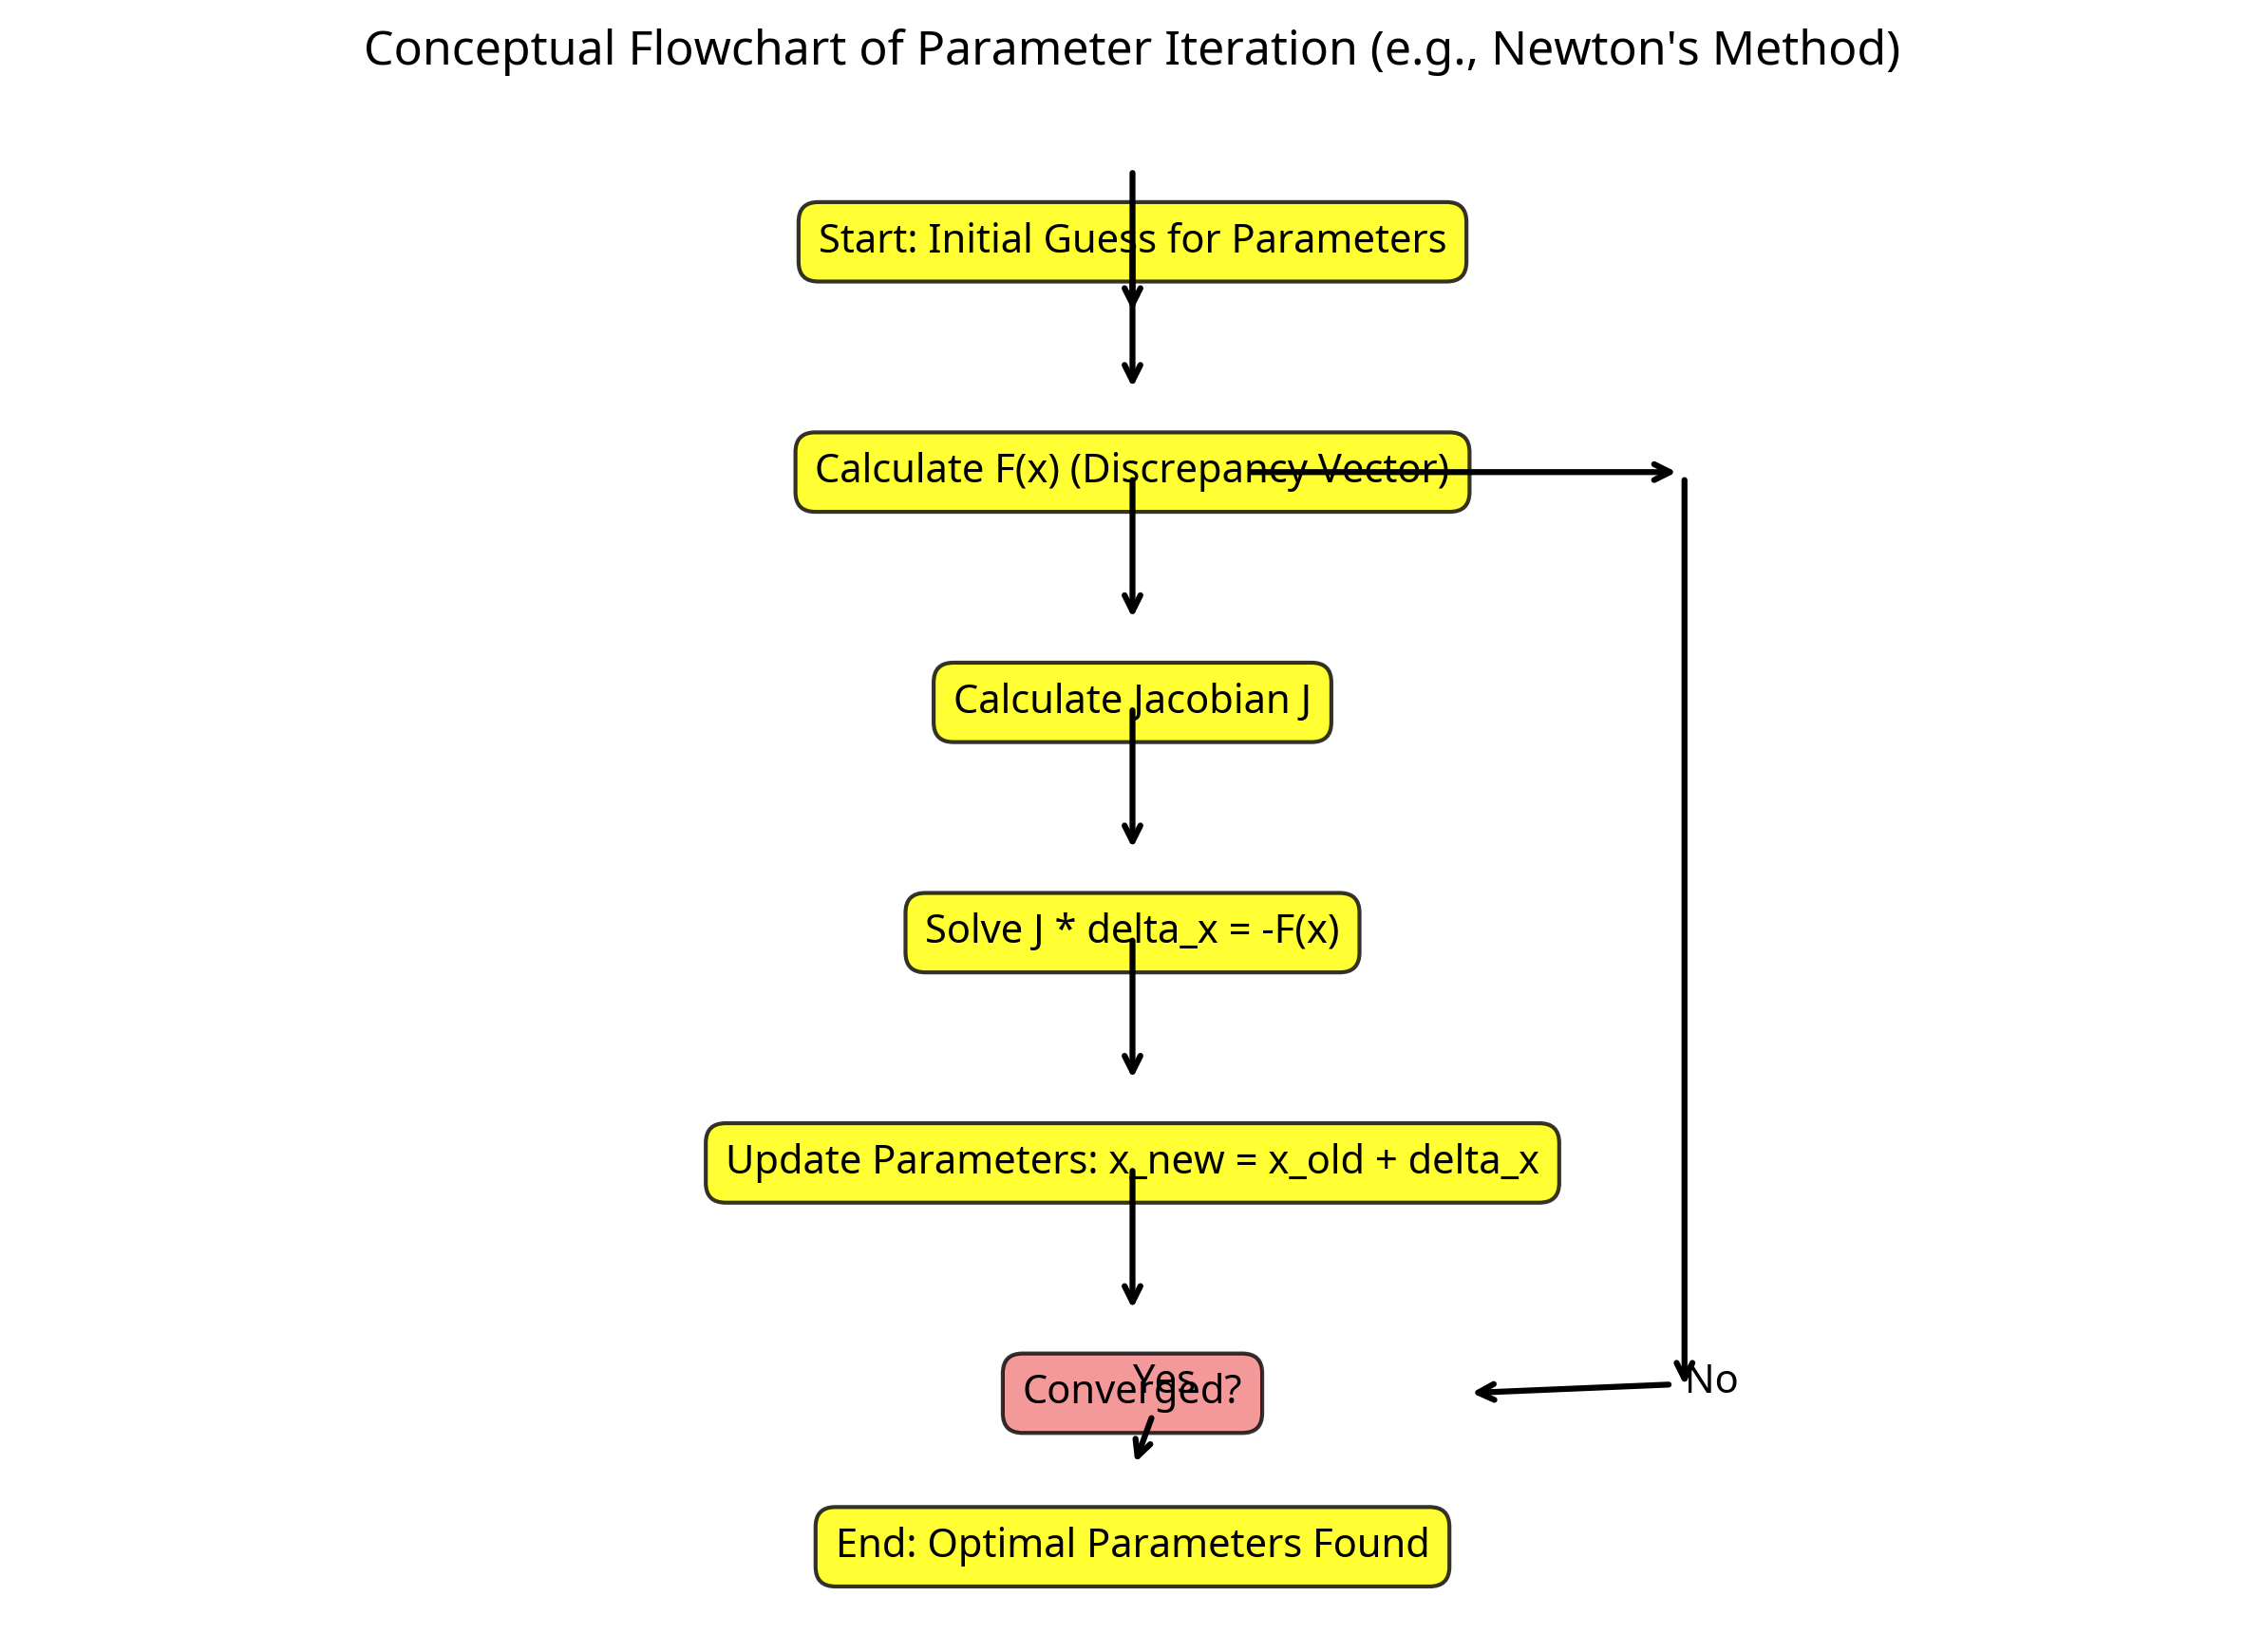
\includegraphics[width=0.9\textwidth]{diagrams/parameter_iteration_flowchart.png}
    \caption{Conceptual flowchart of parameter iteration, illustrating a method like Newton\`s for finding optimal parameters in conformal mapping. The process involves iterative calculation and updating until convergence is achieved.}
    \label{fig:parameter_iteration_flowchart}
\end{figure}


This chapter focuses on various numerical methods for determining the parameters (pre-vertices $w_j$ and constants $C_1, C_2$) in the Schwarz-Christoffel transformation:

\begin{equation}
    \impformula{z(w) = C_1 \int_{w_0}^w \prod_{j=1}^n (t - w_j)^{-\alpha_j} dt + C_2} \label{eq:general_sc_integral}
\end{equation}

Several methods have been developed to tackle this complex problem.

\section{Parameter Method}

The parameter method involves determining the parameters by equating the values of $z(w)$ in the z-plane to the values of the integral evaluated at corresponding points $w_j$ on the v-axis. This leads to a system of simultaneous, nonlinear equations. For instance, by equating ratios of lengths between adjacent vertices, a system of equations can be formed:

\begin{equation}
    \impformula{\frac{\Delta z_{kl}}{\Delta z_{mk}} = \frac{\Delta F_{kl}}{\Delta F_{mk}}} \label{eq:parameter_method_ratio}
\end{equation}

where $\Delta z_{kl}$ represents the distance between vertices $z_k$ and $z_l$, and $\Delta F_{kl}$ is the corresponding integral value. This system can then be solved using optimization techniques, such as minimizing the sum of squared errors.

\section{van Dyke's Method}

Van Dyke's method is particularly useful when an approximate, yet accurate, solution is required in the vicinity of a singular point. It leverages the fact that the factor $(t - w_j)^{-\alpha_j}$ in the Schwarz-Christoffel transformation predominates as the integration approaches the singular point $w_j$. The method provides an approximation for the change in $z$ across an interval containing a singular point:

\begin{equation}
    \impformula{\Delta z_m \approx C_1 \left( \prod_{j \neq m} (w_m - w_j)^{-\alpha_j} \right) \frac{(w^+ - w_m)^{1-\alpha_m} - (w^- - w_m)^{1-\alpha_m}}{1-\alpha_m}} \label{eq:van_dyke_approx}
\end{equation}

However, this method has limitations, particularly when $\alpha_m = 1$ or when singular points are densely packed. It is also less suitable when vertices in the z-plane are at infinity, though symmetry can sometimes be exploited to mitigate this.

\begin{figure}[H]
    \centering
    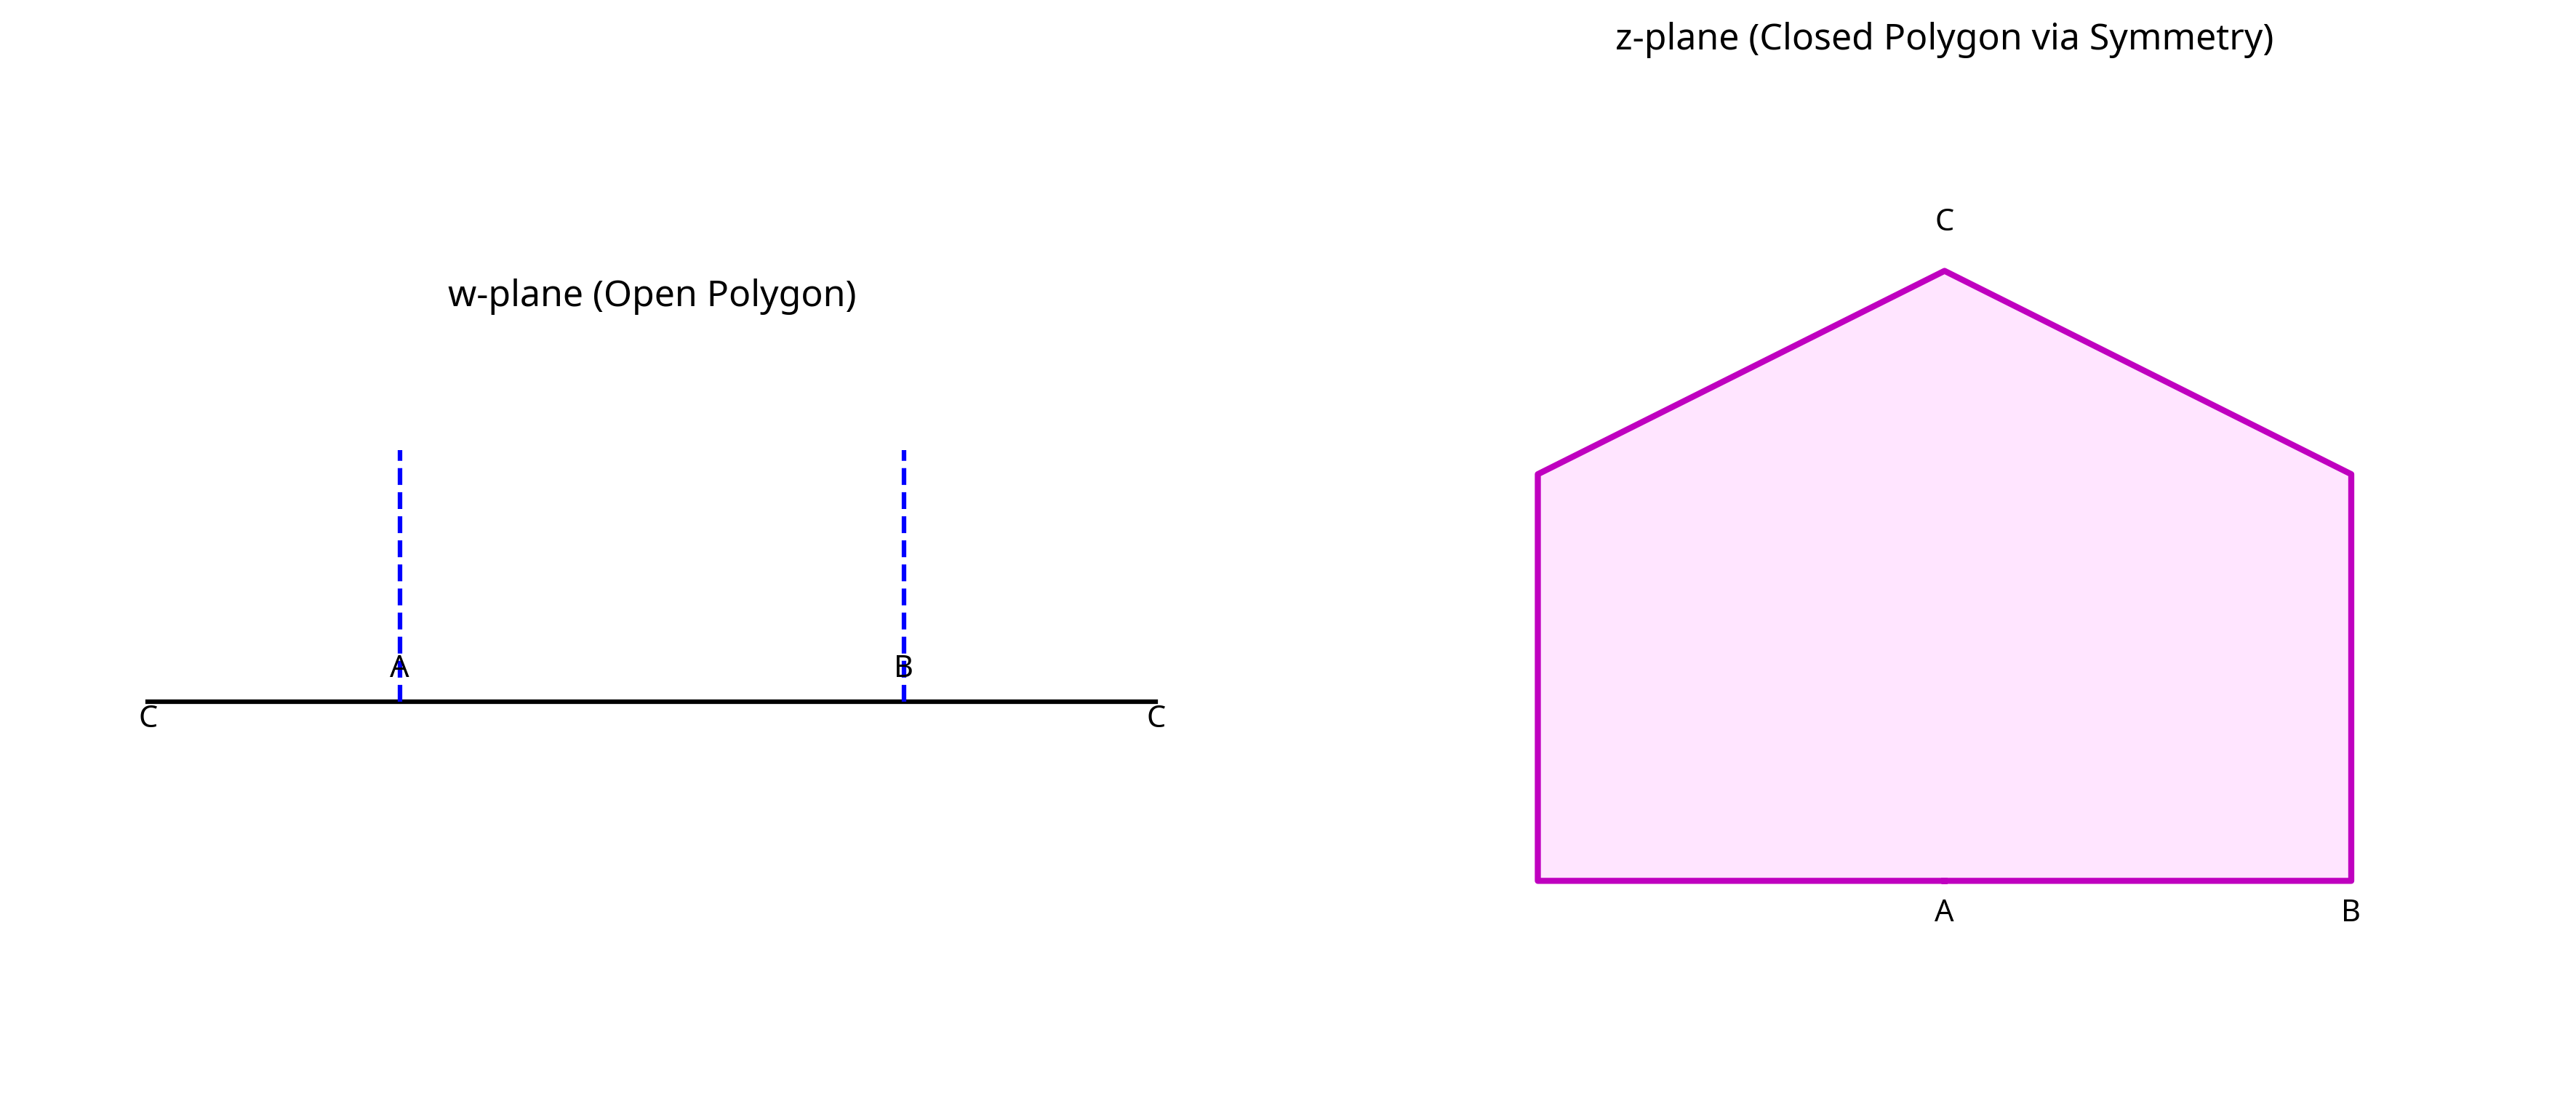
\includegraphics[width=0.7\textwidth]{diagrams/symmetry_avoid_infinity.png}
    \caption{Use of symmetry to avoid vertices at infinity in the z-plane, transforming an open polygon into a symmetric, closed one.}
    \label{fig:symmetry_avoid_infinity}
\end{figure}

\section{Trefethen's Method (SCPACK)}

Trefethen's method, often implemented through software packages like SCPACK, focuses on mapping the polygon in the z-plane onto the unit disk. This approach offers advantages in numerical stability. The pre-vertices $z_j$ are mapped onto the unit circle as $w_j = e^{i\Theta_j}$, and the problem reduces to determining these angles $\Theta_j$. The method employs Gauss-Jacobi quadrature for integral evaluation and an iterative procedure based on Powell's minimization method for solving the nonlinear equations. A key principle is to ensure that singular points are not too close to integration intervals to maintain accuracy.

\section{Foster-Anderson's Method}

Foster-Anderson's method utilizes elliptic functions for the numerical evaluation of the Schwarz-Christoffel integral. This approach provides an alternative mathematical framework for handling the integrals, particularly for complex geometries. The algorithm, published by Warner and Anderson, details the steps for synthesizing a polygon to conform with a desired modulus.

\begin{figure}[H]
    \centering
    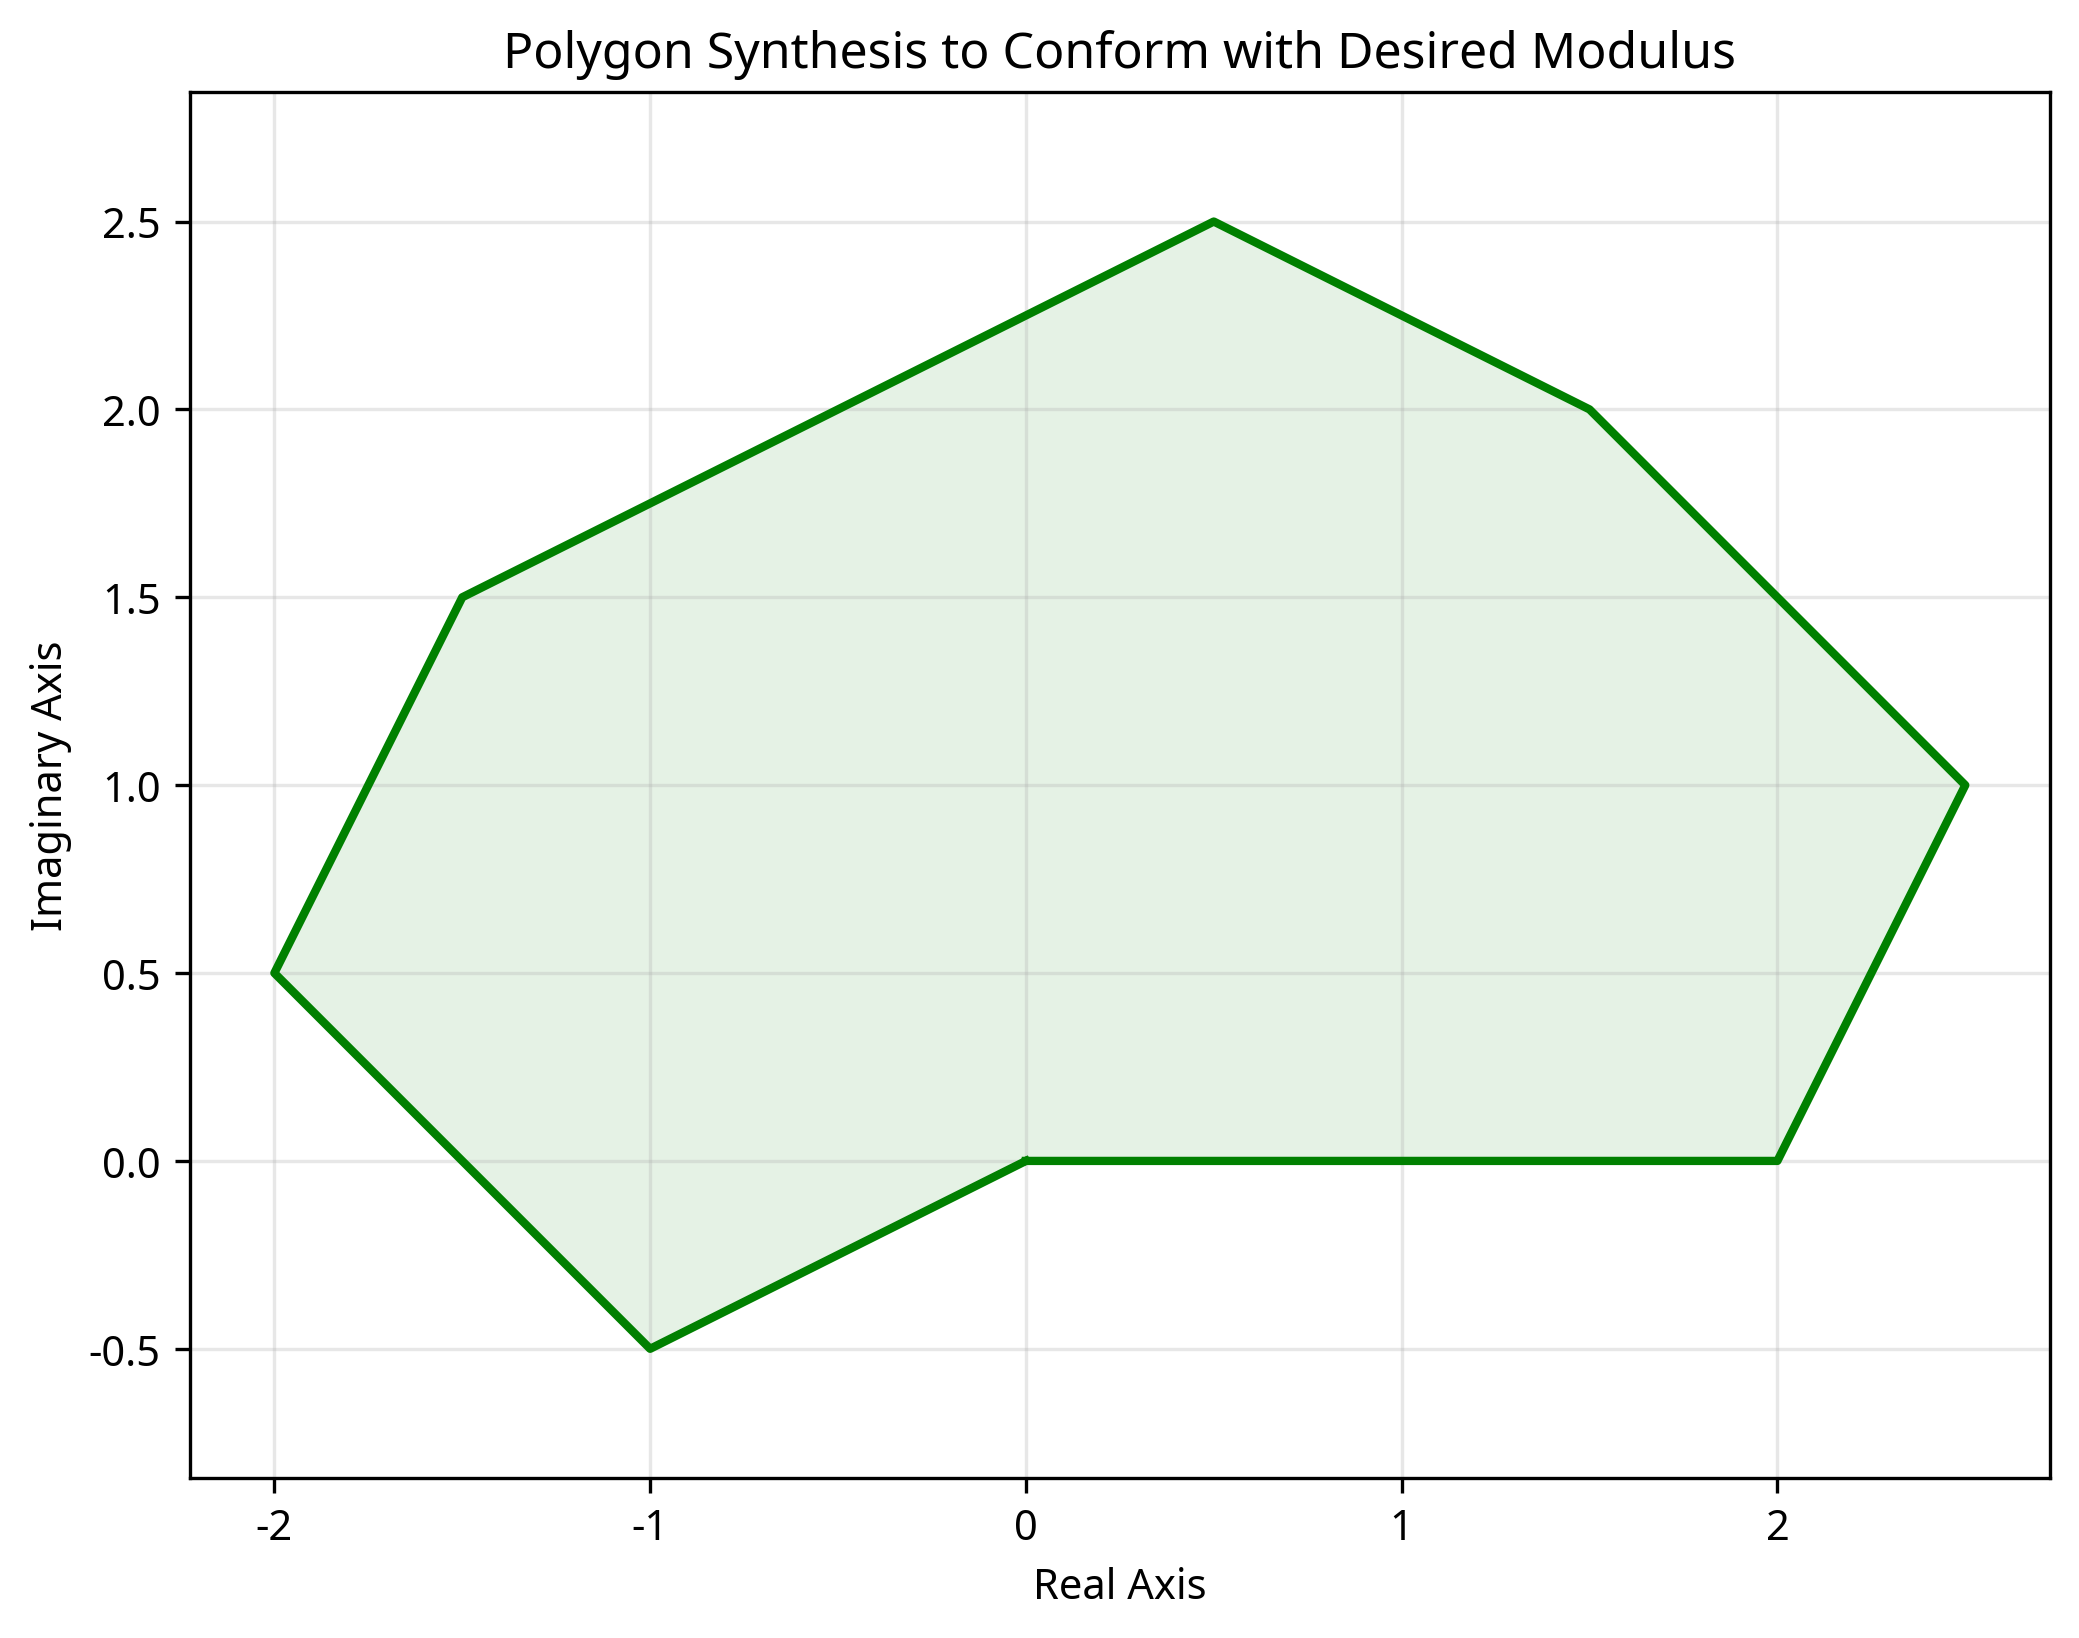
\includegraphics[width=0.7\textwidth]{diagrams/polygon_synthesis.png}
    \caption{Synthesis of a polygon to conform with a desired modulus, often achieved using methods like Foster-Anderson's that leverage elliptic functions.}
    \label{fig:polygon_synthesis}
\end{figure}

\chapter{Conclusion}

This report has provided a comprehensive overview of conformal mapping applications, with a particular emphasis on the Schwarz-Christoffel transformation and associated numerical methods. We have explored the fundamental concepts of the parameter problem, various numerical techniques for solving the complex integrals involved, and specialized methods for handling singularities. Furthermore, the report delved into extremal problems such as the minimum area and minimum boundary problems, highlighting their theoretical underpinnings through the Bergman and Szego kernels, and their numerical solutions via the Ritz method.

The ability of conformal mapping to transform complex geometries into simpler domains makes it an indispensable tool in fields ranging from fluid dynamics and electrostatics to heat transfer and elasticity. The numerical methods discussed, including Newton's method, Trefethen's SCPACK, van Dyke's method, and Foster-Anderson's method, underscore the practical applicability of these theoretical concepts in solving real-world engineering and physics problems. The challenges associated with singularities and the determination of accessory parameters have led to sophisticated computational techniques that ensure accuracy and efficiency.

Future work in this area could involve exploring more advanced numerical algorithms for higher-order polygons, investigating the application of machine learning techniques to predict optimal parameters, or extending these methods to three-dimensional conformal mappings, which remain a significant challenge in computational mathematics.

\end{document}
